\documentclass[twoside]{book}

% Packages required by doxygen
\usepackage{fixltx2e}
\usepackage{calc}
\usepackage{doxygen}
\usepackage[export]{adjustbox} % also loads graphicx
\usepackage{graphicx}
\usepackage[utf8]{inputenc}
\usepackage{makeidx}
\usepackage{multicol}
\usepackage{multirow}
\PassOptionsToPackage{warn}{textcomp}
\usepackage{textcomp}
\usepackage[nointegrals]{wasysym}
\usepackage[table]{xcolor}

% Font selection
\usepackage[T1]{fontenc}
\usepackage[scaled=.90]{helvet}
\usepackage{courier}
\usepackage{amssymb}
\usepackage{sectsty}
\renewcommand{\familydefault}{\sfdefault}
\allsectionsfont{%
  \fontseries{bc}\selectfont%
  \color{darkgray}%
}
\renewcommand{\DoxyLabelFont}{%
  \fontseries{bc}\selectfont%
  \color{darkgray}%
}
\newcommand{\+}{\discretionary{\mbox{\scriptsize$\hookleftarrow$}}{}{}}

% Page & text layout
\usepackage{geometry}
\geometry{%
  a4paper,%
  top=2.5cm,%
  bottom=2.5cm,%
  left=2.5cm,%
  right=2.5cm%
}
\tolerance=750
\hfuzz=15pt
\hbadness=750
\setlength{\emergencystretch}{15pt}
\setlength{\parindent}{0cm}
\setlength{\parskip}{3ex plus 2ex minus 2ex}
\makeatletter
\renewcommand{\paragraph}{%
  \@startsection{paragraph}{4}{0ex}{-1.0ex}{1.0ex}{%
    \normalfont\normalsize\bfseries\SS@parafont%
  }%
}
\renewcommand{\subparagraph}{%
  \@startsection{subparagraph}{5}{0ex}{-1.0ex}{1.0ex}{%
    \normalfont\normalsize\bfseries\SS@subparafont%
  }%
}
\makeatother

% Headers & footers
\usepackage{fancyhdr}
\pagestyle{fancyplain}
\fancyhead[LE]{\fancyplain{}{\bfseries\thepage}}
\fancyhead[CE]{\fancyplain{}{}}
\fancyhead[RE]{\fancyplain{}{\bfseries\leftmark}}
\fancyhead[LO]{\fancyplain{}{\bfseries\rightmark}}
\fancyhead[CO]{\fancyplain{}{}}
\fancyhead[RO]{\fancyplain{}{\bfseries\thepage}}
\fancyfoot[LE]{\fancyplain{}{}}
\fancyfoot[CE]{\fancyplain{}{}}
\fancyfoot[RE]{\fancyplain{}{\bfseries\scriptsize Generated by Doxygen }}
\fancyfoot[LO]{\fancyplain{}{\bfseries\scriptsize Generated by Doxygen }}
\fancyfoot[CO]{\fancyplain{}{}}
\fancyfoot[RO]{\fancyplain{}{}}
\renewcommand{\footrulewidth}{0.4pt}
\renewcommand{\chaptermark}[1]{%
  \markboth{#1}{}%
}
\renewcommand{\sectionmark}[1]{%
  \markright{\thesection\ #1}%
}

% Indices & bibliography
\usepackage{natbib}
\usepackage[titles]{tocloft}
\setcounter{tocdepth}{3}
\setcounter{secnumdepth}{5}
\makeindex

% Hyperlinks (required, but should be loaded last)
\usepackage{ifpdf}
\ifpdf
  \usepackage[pdftex,pagebackref=true]{hyperref}
\else
  \usepackage[ps2pdf,pagebackref=true]{hyperref}
\fi
\hypersetup{%
  colorlinks=true,%
  linkcolor=blue,%
  citecolor=blue,%
  unicode%
}

% Custom commands
\newcommand{\clearemptydoublepage}{%
  \newpage{\pagestyle{empty}\cleardoublepage}%
}

\usepackage{caption}
\captionsetup{labelsep=space,justification=centering,font={bf},singlelinecheck=off,skip=4pt,position=top}

%===== C O N T E N T S =====

\begin{document}

% Titlepage & ToC
\hypersetup{pageanchor=false,
             bookmarksnumbered=true,
             pdfencoding=unicode
            }
\pagenumbering{roman}
\begin{titlepage}
\vspace*{7cm}
\begin{center}%
{\Large My Project \\[1ex]\large Midsemester project of Karan Vivek Bhargava }\\
\vspace*{1cm}
{\large Generated by Doxygen 1.8.11}\\
\end{center}
\end{titlepage}
\clearemptydoublepage
\tableofcontents
\clearemptydoublepage
\pagenumbering{arabic}
\hypersetup{pageanchor=true}

%--- Begin generated contents ---
\chapter{readme}
\label{md_readme}
\hypertarget{md_readme}{}
\section*{E\+N\+P\+M808X -\/ \hyperlink{class_robot}{Robot} Butler }

\href{https://travis-ci.org/karanvivekbhargava/robot-butler-enpm808x}{\tt } \href{https://coveralls.io/github/karanvivekbhargava/robot-butler-enpm808x?branch=master}{\tt } \href{https://opensource.org/licenses/MIT}{\tt } 

 Reference for image\+: \href{http://www.savioke.com/}{\tt link} 

\subsection*{\hyperlink{class_robot}{Robot} Overview}

The Butler product by Acme Robotics is one of its flagship products. It performs best for an environment where things are to be transported to and fro from one area to another. Equipped with a 16\+MP camera and the best of class custom lidar sensor, its the best offering one can hope for. The butler has intelligent algorithms running under its hood which allow it to percieve its environment by using these sensors. This allows the butler to avoid hitting obstacles and helps it serve you better.

\subsection*{New Feature List}

We tirelessly work on our robots so that you don\textquotesingle{}t have to. Our new offerings in software are included below.
\begin{DoxyItemize}
\item Estimation of object distances using camera data\+: While other companies are defining state of the art algorithms on the road, we do it in your workplace. Making our robots 30\% less likely to crash into objects than our competitors.
\item Using lidar to map your environment\+: The butler records its surroundings in 3D so that it can see obstacles before they hit it.
\item Advanced data fusion algorithms\+: Our robots are cool but don\textquotesingle{}t be fooled by their innocent appearance, they work super hard on the inside to crunch numbers faster than ever.
\item Path Planning\+: Using our custom sensors and the fusion technique, we can better plan the paths to avoid obstacles 

 \subsection*{The Camera}
\end{DoxyItemize}

The butler has a 16\+MP front facing camera. Its camera module consists of an F\+P\+GA which can perform custom algorithms at a mind boggling pace. Once the input image arrives, the module does a perspective transform on it. This gives us a birds eye view which is then passed to a thresholder. The binarized image from the thresholder is then used to calculate the probabilities of hitting the nearby obstacles. We use a gaussian probability distribution to compute the same.

The images below show how the camera module is manupulating the data to translate it into a probability. The left image is the input, the center image is the perspective warped image and the right image is the thresholded image after warping. After this I\textquotesingle{}m checking the distances to obstacles with different headding directions. I can use these distances to obtain probabilties using a gaussian distribution. 

   

\subsection*{The Lidar}

The lidar gives a three dimensional point cloud representation of its surroundings. It uses this information and \textquotesingle{}flattens\textquotesingle{} it out. This results in all the points being in some eucledean plane and the robot being the origin. It computes the distances from the obstacles and returns gaussian probabilitites to all the possible heading directions of the robot.

Example\+: Consider that we have a point from the point cloud as below. PS\+: The points are preprocessed to be in the heading directions that we are going to consider. 
\begin{DoxyCode}
1 p = (1, 2, 3)
\end{DoxyCode}
 The points will be flattened at first, this results in the representation of the points on the ground (euclidean plane). 
\begin{DoxyCode}
1 p\_flattened = (1, 2)
\end{DoxyCode}
 We will then compute the distances of the points from the origin (this is where the robot will be at all times) 
\begin{DoxyCode}
1 d = sqrt(1^2 + 2^2)
\end{DoxyCode}
 We then turn these distances into the probabilities of hitting an obstacle by 
\begin{DoxyCode}
1 Probability = C*e^((d-mean)/(2*variance))
\end{DoxyCode}
 Where C is a normalization constant, mean is 0 and variance is tuned according to the data. The lidar outputs these probabilites.

\subsection*{Sensor Fusion}

After the camera and lidar do the hard work of putting the information in a sensible format, the sensor fusion module takes the two readings and selects the higher probability of the two, for each heading direction. Although this might result in some noisy outputs, it gives a high probability of avoiding obstacles.

Example\+: If say we have the incoming probabilities given below where the probabilities correspond to heading directions -\/30, -\/20, -\/10, 10, 20, 30 degrees from current heading direction. 
\begin{DoxyCode}
1 P\_image = [0.1, 0.2, 0.3, 0.4, 0.5, 0.6];
2 P\_lidar = [0.6, 0.5, 0.4, 0.3, 0.2, 0,1];
\end{DoxyCode}
 Fused probability is given by 
\begin{DoxyCode}
1 P\_fusion = max(P\_image, P\_lidar)
\end{DoxyCode}
 Which gives us, 
\begin{DoxyCode}
1 P\_fusion = [0.6, 0.5, 0.4, 0.4, 0.5, 0.6];
\end{DoxyCode}


\subsection*{Path Planning}

The path planner uses the fused sensor output to determine what should be the next heading direction. This is done by selecting the heading direction which results in the least probability of hitting any obstacles.

Example\+: If the incoming fused probabilities are as given below 
\begin{DoxyCode}
1 P\_fused = [0.1, 0.2, 0.0, 0.01, 0.1, 0,3];
\end{DoxyCode}
 Then the path planner can be written mathematically as 
\begin{DoxyCode}
1 direction = argmin\_x( P\_fused[x] )
\end{DoxyCode}
 Then the output of the path planner would be 
\begin{DoxyCode}
1 direction = 2 (index of 0.0)
\end{DoxyCode}


\subsection*{The \hyperlink{class_robot}{Robot}}

The robot is the class which uses all the other modules and creates instances of a camera, lidar, sensor fusion module and path planning module. It then uses the modules to run. 

 



 \subsection*{S\+IP Overview}

Click this link to view the product backlog, time sheets, defect logs and release backlog -\/ \href{https://docs.google.com/spreadsheets/d/1WOvV6iL4gGOF8Qacwj2R3Lom71wziKXEf_UEhdGfOuY/edit?usp=sharing}{\tt link}

Care has been taken to design the S\+IP tasks such that they have a direct relation to the previous tasks. This helps in better time estimation. For instance, the change in time taken for stub implementation is proportional to the change in time taken to implement the methods. This gave me a good idea to rethink about the allotment of time for future tasks. 

 \subsection*{Overview}

The butler software stack has the following dependencies\+:
\begin{DoxyItemize}
\item cmake
\item googletest
\item opencv
\end{DoxyItemize}

\#\# Standard install via command-\/line 
\begin{DoxyCode}
1 git clone --recursive https://github.com/karanvivekbhargava/robot-butler-enpm808x
2 cd <path to repository>
3 mkdir build
4 cd build
5 cmake ..
6 make
7 Run tests: ./test/cpp-test
8 Run program: ./app/shell-app
\end{DoxyCode}


\#\# Building for code coverage (for assignments beginning in Week 4) 
\begin{DoxyCode}
1 sudo apt-get install lcov
2 cmake -D COVERAGE=ON -D CMAKE\_BUILD\_TYPE=Debug ../
3 make
4 make code\_coverage
\end{DoxyCode}
 This generates a index.\+html page in the build/coverage sub-\/directory that can be viewed locally in a web browser.

\subsection*{Working with Eclipse I\+DE}

\subsection*{Installation}

In your Eclipse workspace directory (or create a new one), checkout the repo (and submodules) 
\begin{DoxyCode}
1 mkdir -p ~/workspace
2 cd ~/workspace
3 git clone --recursive https://github.com/karanvivekbhargava/robot-butler-enpm808x
\end{DoxyCode}


In your work directory, use cmake to create an Eclipse project for an \mbox{[}out-\/of-\/source build\mbox{]} of cpp-\/boilerplate


\begin{DoxyCode}
1 cd ~/workspace
2 mkdir -p boilerplate-eclipse
3 cd boilerplate-eclipse
4 cmake -G "Eclipse CDT4 - Unix Makefiles" -D CMAKE\_BUILD\_TYPE=Debug -D CMAKE\_ECLIPSE\_VERSION=4.7.0 -D
       CMAKE\_CXX\_COMPILER\_ARG1=-std=c++14 ../cpp-boilerplate/
\end{DoxyCode}


\subsection*{Import}

Open Eclipse, go to File -\/$>$ Import -\/$>$ General -\/$>$ Existing Projects into Workspace -\/$>$ Select \char`\"{}boilerplate-\/eclipse\char`\"{} directory created previously as root directory -\/$>$ Finish

\section*{Edit}

Source files may be edited under the \char`\"{}\mbox{[}\+Source Directory\mbox{]}\char`\"{} label in the Project Explorer.

\subsection*{Build}

To build the project, in Eclipse, unfold boilerplate-\/eclipse project in Project Explorer, unfold Build Targets, double click on \char`\"{}all\char`\"{} to build all projects.

\subsection*{Run}


\begin{DoxyEnumerate}
\item In Eclipse, right click on the boilerplate-\/eclipse in Project Explorer, select Run As -\/$>$ Local C/\+C++ Application
\item Choose the binaries to run (e.\+g. shell-\/app, cpp-\/test for unit testing)
\end{DoxyEnumerate}

\subsection*{Debug}


\begin{DoxyEnumerate}
\item Set breakpoint in source file (i.\+e. double click in the left margin on the line you want the program to break).
\item In Eclipse, right click on the boilerplate-\/eclipse in Project Explorer, select Debug As -\/$>$ Local C/\+C++ Application, choose the binaries to run (e.\+g. shell-\/app).
\item If prompt to \char`\"{}\+Confirm Perspective Switch\char`\"{}, select yes.
\item Program will break at the breakpoint you set.
\item Press Step Into (F5), Step Over (F6), Step Return (F7) to step/debug your program.
\item Right click on the variable in editor to add watch expression to watch the variable in debugger window.
\item Press Terminate icon to terminate debugging and press C/\+C++ icon to switch back to C/\+C++ perspetive view (or Windows-\/$>$Perspective-\/$>$Open Perspective-\/$>$C/\+C++).
\end{DoxyEnumerate}

\subsection*{Plugins}


\begin{DoxyItemize}
\item Cpp\+Ch\+Eclipse

To install and run cppcheck in Eclipse
\begin{DoxyEnumerate}
\item In Eclipse, go to Window -\/$>$ Preferences -\/$>$ C/\+C++ -\/$>$ cppcheclipse. Set cppcheck binary path to \char`\"{}/usr/bin/cppcheck\char`\"{}.
\item To run C\+P\+P\+Check on a project, right click on the project name in the Project Explorer and choose cppcheck -\/$>$ Run cppcheck.
\end{DoxyEnumerate}
\item Google C++ Sytle

To include and use Google C++ Style formatter in Eclipse
\begin{DoxyEnumerate}
\item In Eclipse, go to Window -\/$>$ Preferences -\/$>$ C/\+C++ -\/$>$ Code Style -\/$>$ Formatter. Import \href{https://raw.githubusercontent.com/google/styleguide/gh-pages/eclipse-cpp-google-style.xml}{\tt eclipse-\/cpp-\/google-\/style} and apply.
\item To use Google C++ style formatter, right click on the source code or folder in Project Explorer and choose Source -\/$>$ Format
\end{DoxyEnumerate}
\item Git

It is possible to manage version control through Eclipse and the git plugin, but it typically requires creating another project. If you\textquotesingle{}re interested in this, try it out yourself. 
\end{DoxyItemize}
\chapter{Hierarchical Index}
\section{Class Hierarchy}
This inheritance list is sorted roughly, but not completely, alphabetically\+:\begin{DoxyCompactList}
\item \contentsline{section}{Camera\+Module}{\pageref{class_camera_module}}{}
\item \contentsline{section}{Lidar\+Module}{\pageref{class_lidar_module}}{}
\item \contentsline{section}{Path\+Planning\+Module}{\pageref{class_path_planning_module}}{}
\item \contentsline{section}{Robot}{\pageref{class_robot}}{}
\item \contentsline{section}{Sensor\+Fusion\+Module}{\pageref{class_sensor_fusion_module}}{}
\item Test\begin{DoxyCompactList}
\item \contentsline{section}{Camera\+Test}{\pageref{class_camera_test}}{}
\item \contentsline{section}{Lidar\+Test}{\pageref{class_lidar_test}}{}
\item \contentsline{section}{Path\+Planning\+Test}{\pageref{class_path_planning_test}}{}
\item \contentsline{section}{Sensor\+Fusion\+Test}{\pageref{class_sensor_fusion_test}}{}
\end{DoxyCompactList}
\end{DoxyCompactList}

\chapter{Class Index}
\section{Class List}
Here are the classes, structs, unions and interfaces with brief descriptions\+:\begin{DoxyCompactList}
\item\contentsline{section}{\hyperlink{class_camera_module}{Camera\+Module} \\*Class for camera module }{\pageref{class_camera_module}}{}
\item\contentsline{section}{\hyperlink{class_camera_test}{Camera\+Test} \\*Class for camera test }{\pageref{class_camera_test}}{}
\item\contentsline{section}{\hyperlink{class_lidar_module}{Lidar\+Module} \\*Class for lidar module }{\pageref{class_lidar_module}}{}
\item\contentsline{section}{\hyperlink{class_lidar_test}{Lidar\+Test} \\*Class for lidar test }{\pageref{class_lidar_test}}{}
\item\contentsline{section}{\hyperlink{class_path_planning_module}{Path\+Planning\+Module} \\*Class for path planning module }{\pageref{class_path_planning_module}}{}
\item\contentsline{section}{\hyperlink{class_path_planning_test}{Path\+Planning\+Test} \\*Class for path planning test }{\pageref{class_path_planning_test}}{}
\item\contentsline{section}{\hyperlink{class_robot}{Robot} \\*Class for robot }{\pageref{class_robot}}{}
\item\contentsline{section}{\hyperlink{class_robot_test}{Robot\+Test} \\*Class for \hyperlink{class_robot}{Robot} test }{\pageref{class_robot_test}}{}
\item\contentsline{section}{\hyperlink{class_sensor_fusion_module}{Sensor\+Fusion\+Module} \\*Class for sensor fusion module }{\pageref{class_sensor_fusion_module}}{}
\item\contentsline{section}{\hyperlink{class_sensor_fusion_test}{Sensor\+Fusion\+Test} \\*Class for sensor fusion test }{\pageref{class_sensor_fusion_test}}{}
\end{DoxyCompactList}

\chapter{File Index}
\section{File List}
Here is a list of all files with brief descriptions\+:\begin{DoxyCompactList}
\item\contentsline{section}{\hyperlink{_8ycm__extra__conf_8py}{.\+ycm\+\_\+extra\+\_\+conf.\+py} }{\pageref{_8ycm__extra__conf_8py}}{}
\item\contentsline{section}{app/\hyperlink{_camera_module_8cpp}{Camera\+Module.\+cpp} \\*E\+N\+P\+M808X, Midsemester project }{\pageref{_camera_module_8cpp}}{}
\item\contentsline{section}{app/\hyperlink{_lidar_module_8cpp}{Lidar\+Module.\+cpp} \\*E\+N\+P\+M808X, Midsemester project }{\pageref{_lidar_module_8cpp}}{}
\item\contentsline{section}{app/\hyperlink{app_2main_8cpp}{main.\+cpp} }{\pageref{app_2main_8cpp}}{}
\item\contentsline{section}{app/\hyperlink{_path_planning_module_8cpp}{Path\+Planning\+Module.\+cpp} \\*E\+N\+P\+M808X, Midsemester project }{\pageref{_path_planning_module_8cpp}}{}
\item\contentsline{section}{app/\hyperlink{_robot_8cpp}{Robot.\+cpp} \\*E\+N\+P\+M808X, Midsemester project }{\pageref{_robot_8cpp}}{}
\item\contentsline{section}{app/\hyperlink{_sensor_fusion_module_8cpp}{Sensor\+Fusion\+Module.\+cpp} \\*E\+N\+P\+M808X, Midsemester project }{\pageref{_sensor_fusion_module_8cpp}}{}
\item\contentsline{section}{include/\hyperlink{_camera_module_8hpp}{Camera\+Module.\+hpp} \\*E\+N\+P\+M808X, Midsemester project }{\pageref{_camera_module_8hpp}}{}
\item\contentsline{section}{include/\hyperlink{_lidar_module_8hpp}{Lidar\+Module.\+hpp} \\*E\+N\+P\+M808X, Midsemester project }{\pageref{_lidar_module_8hpp}}{}
\item\contentsline{section}{include/\hyperlink{_path_planning_module_8hpp}{Path\+Planning\+Module.\+hpp} \\*E\+N\+P\+M808X, Midsemester project }{\pageref{_path_planning_module_8hpp}}{}
\item\contentsline{section}{include/\hyperlink{_robot_8hpp}{Robot.\+hpp} \\*E\+N\+P\+M808X, Midsemester project }{\pageref{_robot_8hpp}}{}
\item\contentsline{section}{include/\hyperlink{_sensor_fusion_module_8hpp}{Sensor\+Fusion\+Module.\+hpp} \\*E\+N\+P\+M808X, Midsemester project }{\pageref{_sensor_fusion_module_8hpp}}{}
\item\contentsline{section}{test/\hyperlink{_camera_test_8cpp}{Camera\+Test.\+cpp} \\*E\+N\+P\+M808X, Midsemester project }{\pageref{_camera_test_8cpp}}{}
\item\contentsline{section}{test/\hyperlink{_lidar_test_8cpp}{Lidar\+Test.\+cpp} \\*E\+N\+P\+M808X, Midsemester project }{\pageref{_lidar_test_8cpp}}{}
\item\contentsline{section}{test/\hyperlink{test_2main_8cpp}{main.\+cpp} }{\pageref{test_2main_8cpp}}{}
\item\contentsline{section}{test/\hyperlink{_path_planning_test_8cpp}{Path\+Planning\+Test.\+cpp} \\*E\+N\+P\+M808X, Midsemester project }{\pageref{_path_planning_test_8cpp}}{}
\item\contentsline{section}{test/\hyperlink{_robot_test_8cpp}{Robot\+Test.\+cpp} \\*E\+N\+P\+M808X, Midsemester project }{\pageref{_robot_test_8cpp}}{}
\item\contentsline{section}{test/\hyperlink{_sensor_fusion_test_8cpp}{Sensor\+Fusion\+Test.\+cpp} }{\pageref{_sensor_fusion_test_8cpp}}{}
\end{DoxyCompactList}

\chapter{Class Documentation}
\hypertarget{class_camera_module}{}\section{Camera\+Module Class Reference}
\label{class_camera_module}\index{Camera\+Module@{Camera\+Module}}


Class for camera module.  




{\ttfamily \#include $<$Camera\+Module.\+hpp$>$}

\subsection*{Public Member Functions}
\begin{DoxyCompactItemize}
\item 
\hyperlink{class_camera_module_aee54ebbc4116cf63c1e9a95987d779a0}{Camera\+Module} ()
\begin{DoxyCompactList}\small\item\em Constructor. \end{DoxyCompactList}\item 
\hyperlink{class_camera_module_a04bd90027432f057e9b12d1c601c8fcb}{$\sim$\+Camera\+Module} ()
\begin{DoxyCompactList}\small\item\em Destroys the object. \end{DoxyCompactList}\item 
void \hyperlink{class_camera_module_abaf1518284d63d4e30d25e86d116856f}{set\+Input} (cv\+::\+Mat input)
\begin{DoxyCompactList}\small\item\em Sets the input image. \end{DoxyCompactList}\item 
bool \hyperlink{class_camera_module_aa160cacc20eb07d54e1130234f339a46}{get\+Diagnostic} ()
\begin{DoxyCompactList}\small\item\em Gets the diagnostic. \end{DoxyCompactList}\item 
void \hyperlink{class_camera_module_a1b442eae9cbc3101ed73d5dffbeb49f3}{warp\+And\+Binarize} ()
\begin{DoxyCompactList}\small\item\em Warps the image and binarizes it. \end{DoxyCompactList}\item 
std\+::vector$<$ float $>$ \hyperlink{class_camera_module_adefaf0a7a6f6d78cc6d8ff0d15ff77f4}{compute\+Probabilities} ()
\begin{DoxyCompactList}\small\item\em Calculates the probabilities. \end{DoxyCompactList}\end{DoxyCompactItemize}


\subsection{Detailed Description}
Class for camera module. 

\subsection{Constructor \& Destructor Documentation}
\index{Camera\+Module@{Camera\+Module}!Camera\+Module@{Camera\+Module}}
\index{Camera\+Module@{Camera\+Module}!Camera\+Module@{Camera\+Module}}
\subsubsection[{\texorpdfstring{Camera\+Module()}{CameraModule()}}]{\setlength{\rightskip}{0pt plus 5cm}Camera\+Module\+::\+Camera\+Module (
\begin{DoxyParamCaption}
{}
\end{DoxyParamCaption}
)}\hypertarget{class_camera_module_aee54ebbc4116cf63c1e9a95987d779a0}{}\label{class_camera_module_aee54ebbc4116cf63c1e9a95987d779a0}


Constructor. 

Constructs the object. \index{Camera\+Module@{Camera\+Module}!````~Camera\+Module@{$\sim$\+Camera\+Module}}
\index{````~Camera\+Module@{$\sim$\+Camera\+Module}!Camera\+Module@{Camera\+Module}}
\subsubsection[{\texorpdfstring{$\sim$\+Camera\+Module()}{~CameraModule()}}]{\setlength{\rightskip}{0pt plus 5cm}Camera\+Module\+::$\sim$\+Camera\+Module (
\begin{DoxyParamCaption}
{}
\end{DoxyParamCaption}
)}\hypertarget{class_camera_module_a04bd90027432f057e9b12d1c601c8fcb}{}\label{class_camera_module_a04bd90027432f057e9b12d1c601c8fcb}


Destroys the object. 



\subsection{Member Function Documentation}
\index{Camera\+Module@{Camera\+Module}!compute\+Probabilities@{compute\+Probabilities}}
\index{compute\+Probabilities@{compute\+Probabilities}!Camera\+Module@{Camera\+Module}}
\subsubsection[{\texorpdfstring{compute\+Probabilities()}{computeProbabilities()}}]{\setlength{\rightskip}{0pt plus 5cm}std\+::vector$<$ float $>$ Camera\+Module\+::compute\+Probabilities (
\begin{DoxyParamCaption}
{}
\end{DoxyParamCaption}
)}\hypertarget{class_camera_module_adefaf0a7a6f6d78cc6d8ff0d15ff77f4}{}\label{class_camera_module_adefaf0a7a6f6d78cc6d8ff0d15ff77f4}


Calculates the probabilities. 

\begin{DoxyReturn}{Returns}
The probabilities for heading directions. 
\end{DoxyReturn}
\index{Camera\+Module@{Camera\+Module}!get\+Diagnostic@{get\+Diagnostic}}
\index{get\+Diagnostic@{get\+Diagnostic}!Camera\+Module@{Camera\+Module}}
\subsubsection[{\texorpdfstring{get\+Diagnostic()}{getDiagnostic()}}]{\setlength{\rightskip}{0pt plus 5cm}bool Camera\+Module\+::get\+Diagnostic (
\begin{DoxyParamCaption}
{}
\end{DoxyParamCaption}
)}\hypertarget{class_camera_module_aa160cacc20eb07d54e1130234f339a46}{}\label{class_camera_module_aa160cacc20eb07d54e1130234f339a46}


Gets the diagnostic. 

\begin{DoxyReturn}{Returns}
The diagnostic truth value. 
\end{DoxyReturn}
\index{Camera\+Module@{Camera\+Module}!set\+Input@{set\+Input}}
\index{set\+Input@{set\+Input}!Camera\+Module@{Camera\+Module}}
\subsubsection[{\texorpdfstring{set\+Input(cv\+::\+Mat input)}{setInput(cv::Mat input)}}]{\setlength{\rightskip}{0pt plus 5cm}void Camera\+Module\+::set\+Input (
\begin{DoxyParamCaption}
\item[{cv\+::\+Mat}]{input}
\end{DoxyParamCaption}
)}\hypertarget{class_camera_module_abaf1518284d63d4e30d25e86d116856f}{}\label{class_camera_module_abaf1518284d63d4e30d25e86d116856f}


Sets the input image. 


\begin{DoxyParams}[1]{Parameters}
\mbox{\tt in}  & {\em input} & The input image \\
\hline
\end{DoxyParams}
\index{Camera\+Module@{Camera\+Module}!warp\+And\+Binarize@{warp\+And\+Binarize}}
\index{warp\+And\+Binarize@{warp\+And\+Binarize}!Camera\+Module@{Camera\+Module}}
\subsubsection[{\texorpdfstring{warp\+And\+Binarize()}{warpAndBinarize()}}]{\setlength{\rightskip}{0pt plus 5cm}void Camera\+Module\+::warp\+And\+Binarize (
\begin{DoxyParamCaption}
{}
\end{DoxyParamCaption}
)}\hypertarget{class_camera_module_a1b442eae9cbc3101ed73d5dffbeb49f3}{}\label{class_camera_module_a1b442eae9cbc3101ed73d5dffbeb49f3}


Warps the image and binarizes it. 



The documentation for this class was generated from the following files\+:\begin{DoxyCompactItemize}
\item 
include/\hyperlink{_camera_module_8hpp}{Camera\+Module.\+hpp}\item 
app/\hyperlink{_camera_module_8cpp}{Camera\+Module.\+cpp}\end{DoxyCompactItemize}

\hypertarget{class_camera_test}{}\section{Camera\+Test Class Reference}
\label{class_camera_test}\index{Camera\+Test@{Camera\+Test}}


Class for camera test.  




Inheritance diagram for Camera\+Test\+:
\nopagebreak
\begin{figure}[H]
\begin{center}
\leavevmode
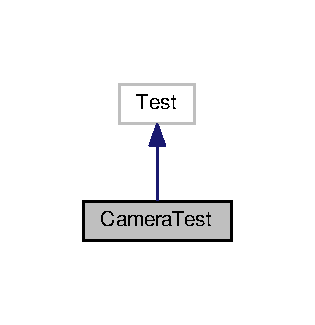
\includegraphics[width=151pt]{class_camera_test__inherit__graph}
\end{center}
\end{figure}


Collaboration diagram for Camera\+Test\+:
\nopagebreak
\begin{figure}[H]
\begin{center}
\leavevmode
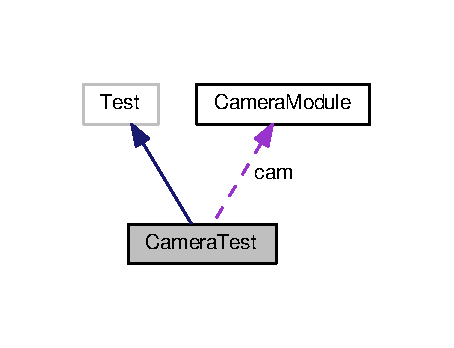
\includegraphics[width=218pt]{class_camera_test__coll__graph}
\end{center}
\end{figure}
\subsection*{Protected Attributes}
\begin{DoxyCompactItemize}
\item 
\hyperlink{class_camera_module}{Camera\+Module} {\bfseries cam}\hypertarget{class_camera_test_a76aa7e4350e4b5773e5641ffa837b100}{}\label{class_camera_test_a76aa7e4350e4b5773e5641ffa837b100}

\end{DoxyCompactItemize}


\subsection{Detailed Description}
Class for camera test. 

Definition at line 22 of file Camera\+Test.\+cpp.



The documentation for this class was generated from the following file\+:\begin{DoxyCompactItemize}
\item 
test/Camera\+Test.\+cpp\end{DoxyCompactItemize}

\hypertarget{class_lidar_module}{}\section{Lidar\+Module Class Reference}
\label{class_lidar_module}\index{Lidar\+Module@{Lidar\+Module}}


Class for lidar module.  




{\ttfamily \#include $<$Lidar\+Module.\+hpp$>$}

\subsection*{Public Member Functions}
\begin{DoxyCompactItemize}
\item 
\hyperlink{class_lidar_module_aaebef565e883b9254ab61d4ba45a19ec}{Lidar\+Module} ()
\begin{DoxyCompactList}\small\item\em Constructor. \end{DoxyCompactList}\item 
\hyperlink{class_lidar_module_a9f76d762ad58356a109e6ca68e9ab34c}{$\sim$\+Lidar\+Module} ()\hypertarget{class_lidar_module_a9f76d762ad58356a109e6ca68e9ab34c}{}\label{class_lidar_module_a9f76d762ad58356a109e6ca68e9ab34c}

\begin{DoxyCompactList}\small\item\em Destroys the object. \end{DoxyCompactList}\item 
void \hyperlink{class_lidar_module_a05318b0c70f04e9f7e9ec7896c3590cf}{set\+Input} (std\+::vector$<$ std\+::vector$<$ float $>$$>$ input)
\begin{DoxyCompactList}\small\item\em Sets the input. \end{DoxyCompactList}\item 
bool \hyperlink{class_lidar_module_a60f2786b71f6baa0756a2355eb1c908a}{get\+Diagnostic} ()
\begin{DoxyCompactList}\small\item\em Gets the diagnostic. \end{DoxyCompactList}\item 
void \hyperlink{class_lidar_module_a9e968b3f52665b2ec1aaae41122b4d0e}{flatten} ()\hypertarget{class_lidar_module_a9e968b3f52665b2ec1aaae41122b4d0e}{}\label{class_lidar_module_a9e968b3f52665b2ec1aaae41122b4d0e}

\begin{DoxyCompactList}\small\item\em Project the points onto the ground. \end{DoxyCompactList}\item 
std\+::vector$<$ float $>$ \hyperlink{class_lidar_module_aeb655e2c122dc36715f013b92689bda6}{compute\+Probabilities} ()
\begin{DoxyCompactList}\small\item\em Calculates the probabilities. \end{DoxyCompactList}\end{DoxyCompactItemize}


\subsection{Detailed Description}
Class for lidar module. 

Definition at line 26 of file Lidar\+Module.\+hpp.



\subsection{Constructor \& Destructor Documentation}
\index{Lidar\+Module@{Lidar\+Module}!Lidar\+Module@{Lidar\+Module}}
\index{Lidar\+Module@{Lidar\+Module}!Lidar\+Module@{Lidar\+Module}}
\subsubsection[{\texorpdfstring{Lidar\+Module()}{LidarModule()}}]{\setlength{\rightskip}{0pt plus 5cm}Lidar\+Module\+::\+Lidar\+Module (
\begin{DoxyParamCaption}
{}
\end{DoxyParamCaption}
)}\hypertarget{class_lidar_module_aaebef565e883b9254ab61d4ba45a19ec}{}\label{class_lidar_module_aaebef565e883b9254ab61d4ba45a19ec}


Constructor. 

Constructs the object. 

Definition at line 22 of file Lidar\+Module.\+cpp.



\subsection{Member Function Documentation}
\index{Lidar\+Module@{Lidar\+Module}!compute\+Probabilities@{compute\+Probabilities}}
\index{compute\+Probabilities@{compute\+Probabilities}!Lidar\+Module@{Lidar\+Module}}
\subsubsection[{\texorpdfstring{compute\+Probabilities()}{computeProbabilities()}}]{\setlength{\rightskip}{0pt plus 5cm}std\+::vector$<$ float $>$ Lidar\+Module\+::compute\+Probabilities (
\begin{DoxyParamCaption}
{}
\end{DoxyParamCaption}
)}\hypertarget{class_lidar_module_aeb655e2c122dc36715f013b92689bda6}{}\label{class_lidar_module_aeb655e2c122dc36715f013b92689bda6}


Calculates the probabilities. 

\begin{DoxyReturn}{Returns}
The probabilities for heading directions. 
\end{DoxyReturn}


Definition at line 85 of file Lidar\+Module.\+cpp.

\index{Lidar\+Module@{Lidar\+Module}!get\+Diagnostic@{get\+Diagnostic}}
\index{get\+Diagnostic@{get\+Diagnostic}!Lidar\+Module@{Lidar\+Module}}
\subsubsection[{\texorpdfstring{get\+Diagnostic()}{getDiagnostic()}}]{\setlength{\rightskip}{0pt plus 5cm}bool Lidar\+Module\+::get\+Diagnostic (
\begin{DoxyParamCaption}
{}
\end{DoxyParamCaption}
)}\hypertarget{class_lidar_module_a60f2786b71f6baa0756a2355eb1c908a}{}\label{class_lidar_module_a60f2786b71f6baa0756a2355eb1c908a}


Gets the diagnostic. 

\begin{DoxyReturn}{Returns}
The diagnostic truth value. 
\end{DoxyReturn}


Definition at line 62 of file Lidar\+Module.\+cpp.

\index{Lidar\+Module@{Lidar\+Module}!set\+Input@{set\+Input}}
\index{set\+Input@{set\+Input}!Lidar\+Module@{Lidar\+Module}}
\subsubsection[{\texorpdfstring{set\+Input(std\+::vector$<$ std\+::vector$<$ float $>$$>$ input)}{setInput(std::vector< std::vector< float >> input)}}]{\setlength{\rightskip}{0pt plus 5cm}void Lidar\+Module\+::set\+Input (
\begin{DoxyParamCaption}
\item[{std\+::vector$<$ std\+::vector$<$ float $>$$>$}]{input}
\end{DoxyParamCaption}
)}\hypertarget{class_lidar_module_a05318b0c70f04e9f7e9ec7896c3590cf}{}\label{class_lidar_module_a05318b0c70f04e9f7e9ec7896c3590cf}


Sets the input. 

Sets the input image.


\begin{DoxyParams}[1]{Parameters}
\mbox{\tt in}  & {\em input} & The input\\
\hline
\mbox{\tt in}  & {\em input} & The input image \\
\hline
\end{DoxyParams}


Definition at line 53 of file Lidar\+Module.\+cpp.



The documentation for this class was generated from the following files\+:\begin{DoxyCompactItemize}
\item 
include/\hyperlink{_lidar_module_8hpp}{Lidar\+Module.\+hpp}\item 
app/\hyperlink{_lidar_module_8cpp}{Lidar\+Module.\+cpp}\end{DoxyCompactItemize}

\hypertarget{class_lidar_test}{}\section{Lidar\+Test Class Reference}
\label{class_lidar_test}\index{Lidar\+Test@{Lidar\+Test}}


Class for lidar test.  




Inheritance diagram for Lidar\+Test\+:
\nopagebreak
\begin{figure}[H]
\begin{center}
\leavevmode
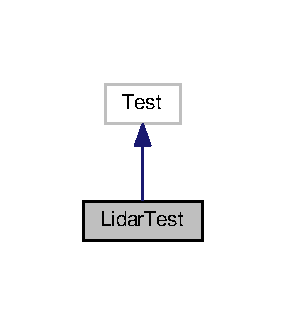
\includegraphics[width=137pt]{class_lidar_test__inherit__graph}
\end{center}
\end{figure}


Collaboration diagram for Lidar\+Test\+:
\nopagebreak
\begin{figure}[H]
\begin{center}
\leavevmode
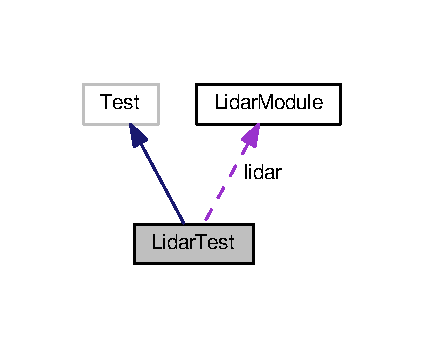
\includegraphics[width=204pt]{class_lidar_test__coll__graph}
\end{center}
\end{figure}
\subsection*{Protected Attributes}
\begin{DoxyCompactItemize}
\item 
\hyperlink{class_lidar_module}{Lidar\+Module} {\bfseries lidar}\hypertarget{class_lidar_test_ab19e318f3d99df132e015dd8c77c4898}{}\label{class_lidar_test_ab19e318f3d99df132e015dd8c77c4898}

\end{DoxyCompactItemize}


\subsection{Detailed Description}
Class for lidar test. 

Definition at line 22 of file Lidar\+Test.\+cpp.



The documentation for this class was generated from the following file\+:\begin{DoxyCompactItemize}
\item 
test/\hyperlink{_lidar_test_8cpp}{Lidar\+Test.\+cpp}\end{DoxyCompactItemize}

\hypertarget{class_path_planning_module}{}\section{Path\+Planning\+Module Class Reference}
\label{class_path_planning_module}\index{Path\+Planning\+Module@{Path\+Planning\+Module}}


Class for path planning module.  




{\ttfamily \#include $<$Path\+Planning\+Module.\+hpp$>$}

\subsection*{Public Member Functions}
\begin{DoxyCompactItemize}
\item 
\hyperlink{class_path_planning_module_a45510d19b199ab89cecc1bf6e8b252eb}{Path\+Planning\+Module} ()
\begin{DoxyCompactList}\small\item\em Constructor. \end{DoxyCompactList}\item 
\hyperlink{class_path_planning_module_acc73ccfa18e08a1771b72bb418d96258}{$\sim$\+Path\+Planning\+Module} ()\hypertarget{class_path_planning_module_acc73ccfa18e08a1771b72bb418d96258}{}\label{class_path_planning_module_acc73ccfa18e08a1771b72bb418d96258}

\begin{DoxyCompactList}\small\item\em Destroys the object. \end{DoxyCompactList}\item 
void \hyperlink{class_path_planning_module_ab44f3d8c24aa57a71ceac2eb71c09c2d}{set\+Heading\+Direction} (int input)
\begin{DoxyCompactList}\small\item\em Sets the heading direction. \end{DoxyCompactList}\item 
bool \hyperlink{class_path_planning_module_a19d31df2f1edafc25580c0c07151e014}{get\+Diagnostic} ()
\begin{DoxyCompactList}\small\item\em Gets the diagnostic. \end{DoxyCompactList}\item 
int \hyperlink{class_path_planning_module_a9aa558d9c088584cbaf37ecede8890b9}{get\+Heading\+Direction} ()
\begin{DoxyCompactList}\small\item\em Gets the heading direction. \end{DoxyCompactList}\item 
void \hyperlink{class_path_planning_module_ae760345016ddc0c7b9381f86240a6ddf}{modify\+Heading\+Direction} (std\+::vector$<$ float $>$ probabilities)
\begin{DoxyCompactList}\small\item\em Modify the heading direction. \end{DoxyCompactList}\end{DoxyCompactItemize}


\subsection{Detailed Description}
Class for path planning module. 

Definition at line 25 of file Path\+Planning\+Module.\+hpp.



\subsection{Constructor \& Destructor Documentation}
\index{Path\+Planning\+Module@{Path\+Planning\+Module}!Path\+Planning\+Module@{Path\+Planning\+Module}}
\index{Path\+Planning\+Module@{Path\+Planning\+Module}!Path\+Planning\+Module@{Path\+Planning\+Module}}
\subsubsection[{\texorpdfstring{Path\+Planning\+Module()}{PathPlanningModule()}}]{\setlength{\rightskip}{0pt plus 5cm}Path\+Planning\+Module\+::\+Path\+Planning\+Module (
\begin{DoxyParamCaption}
{}
\end{DoxyParamCaption}
)}\hypertarget{class_path_planning_module_a45510d19b199ab89cecc1bf6e8b252eb}{}\label{class_path_planning_module_a45510d19b199ab89cecc1bf6e8b252eb}


Constructor. 

Constructs the object. 

Definition at line 22 of file Path\+Planning\+Module.\+cpp.



\subsection{Member Function Documentation}
\index{Path\+Planning\+Module@{Path\+Planning\+Module}!get\+Diagnostic@{get\+Diagnostic}}
\index{get\+Diagnostic@{get\+Diagnostic}!Path\+Planning\+Module@{Path\+Planning\+Module}}
\subsubsection[{\texorpdfstring{get\+Diagnostic()}{getDiagnostic()}}]{\setlength{\rightskip}{0pt plus 5cm}bool Path\+Planning\+Module\+::get\+Diagnostic (
\begin{DoxyParamCaption}
{}
\end{DoxyParamCaption}
)}\hypertarget{class_path_planning_module_a19d31df2f1edafc25580c0c07151e014}{}\label{class_path_planning_module_a19d31df2f1edafc25580c0c07151e014}


Gets the diagnostic. 

\begin{DoxyReturn}{Returns}
The diagnostic truth value. 
\end{DoxyReturn}


Definition at line 45 of file Path\+Planning\+Module.\+cpp.

\index{Path\+Planning\+Module@{Path\+Planning\+Module}!get\+Heading\+Direction@{get\+Heading\+Direction}}
\index{get\+Heading\+Direction@{get\+Heading\+Direction}!Path\+Planning\+Module@{Path\+Planning\+Module}}
\subsubsection[{\texorpdfstring{get\+Heading\+Direction()}{getHeadingDirection()}}]{\setlength{\rightskip}{0pt plus 5cm}int Path\+Planning\+Module\+::get\+Heading\+Direction (
\begin{DoxyParamCaption}
{}
\end{DoxyParamCaption}
)}\hypertarget{class_path_planning_module_a9aa558d9c088584cbaf37ecede8890b9}{}\label{class_path_planning_module_a9aa558d9c088584cbaf37ecede8890b9}


Gets the heading direction. 

\begin{DoxyReturn}{Returns}
The heading direction. 
\end{DoxyReturn}


Definition at line 54 of file Path\+Planning\+Module.\+cpp.

\index{Path\+Planning\+Module@{Path\+Planning\+Module}!modify\+Heading\+Direction@{modify\+Heading\+Direction}}
\index{modify\+Heading\+Direction@{modify\+Heading\+Direction}!Path\+Planning\+Module@{Path\+Planning\+Module}}
\subsubsection[{\texorpdfstring{modify\+Heading\+Direction(std\+::vector$<$ float $>$ probabilities)}{modifyHeadingDirection(std::vector< float > probabilities)}}]{\setlength{\rightskip}{0pt plus 5cm}void Path\+Planning\+Module\+::modify\+Heading\+Direction (
\begin{DoxyParamCaption}
\item[{std\+::vector$<$ float $>$}]{probabilities}
\end{DoxyParamCaption}
)}\hypertarget{class_path_planning_module_ae760345016ddc0c7b9381f86240a6ddf}{}\label{class_path_planning_module_ae760345016ddc0c7b9381f86240a6ddf}


Modify the heading direction. 


\begin{DoxyParams}[1]{Parameters}
\mbox{\tt in}  & {\em probabilities} & The probabilities \\
\hline
\end{DoxyParams}


Definition at line 63 of file Path\+Planning\+Module.\+cpp.

\index{Path\+Planning\+Module@{Path\+Planning\+Module}!set\+Heading\+Direction@{set\+Heading\+Direction}}
\index{set\+Heading\+Direction@{set\+Heading\+Direction}!Path\+Planning\+Module@{Path\+Planning\+Module}}
\subsubsection[{\texorpdfstring{set\+Heading\+Direction(int input)}{setHeadingDirection(int input)}}]{\setlength{\rightskip}{0pt plus 5cm}void Path\+Planning\+Module\+::set\+Heading\+Direction (
\begin{DoxyParamCaption}
\item[{int}]{input}
\end{DoxyParamCaption}
)}\hypertarget{class_path_planning_module_ab44f3d8c24aa57a71ceac2eb71c09c2d}{}\label{class_path_planning_module_ab44f3d8c24aa57a71ceac2eb71c09c2d}


Sets the heading direction. 


\begin{DoxyParams}[1]{Parameters}
\mbox{\tt in}  & {\em input} & The input \\
\hline
\end{DoxyParams}


Definition at line 36 of file Path\+Planning\+Module.\+cpp.



The documentation for this class was generated from the following files\+:\begin{DoxyCompactItemize}
\item 
include/\hyperlink{_path_planning_module_8hpp}{Path\+Planning\+Module.\+hpp}\item 
app/\hyperlink{_path_planning_module_8cpp}{Path\+Planning\+Module.\+cpp}\end{DoxyCompactItemize}

\hypertarget{class_path_planning_test}{}\section{Path\+Planning\+Test Class Reference}
\label{class_path_planning_test}\index{Path\+Planning\+Test@{Path\+Planning\+Test}}


Class for path planning test.  




Inheritance diagram for Path\+Planning\+Test\+:
\nopagebreak
\begin{figure}[H]
\begin{center}
\leavevmode
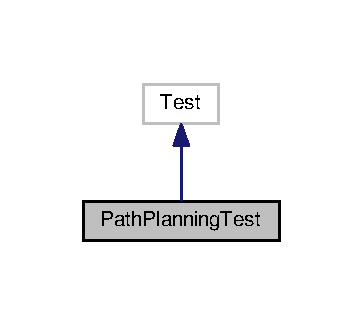
\includegraphics[width=174pt]{class_path_planning_test__inherit__graph}
\end{center}
\end{figure}


Collaboration diagram for Path\+Planning\+Test\+:
\nopagebreak
\begin{figure}[H]
\begin{center}
\leavevmode
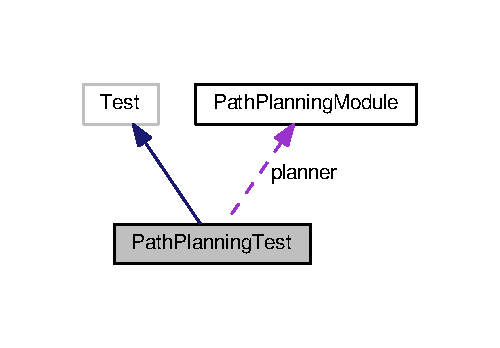
\includegraphics[width=240pt]{class_path_planning_test__coll__graph}
\end{center}
\end{figure}
\subsection*{Protected Attributes}
\begin{DoxyCompactItemize}
\item 
\hyperlink{class_path_planning_module}{Path\+Planning\+Module} \hyperlink{class_path_planning_test_af307c6073040bffa9d602969d81ae254}{planner}
\end{DoxyCompactItemize}


\subsection{Detailed Description}
Class for path planning test. 

\subsection{Member Data Documentation}
\index{Path\+Planning\+Test@{Path\+Planning\+Test}!planner@{planner}}
\index{planner@{planner}!Path\+Planning\+Test@{Path\+Planning\+Test}}
\subsubsection[{\texorpdfstring{planner}{planner}}]{\setlength{\rightskip}{0pt plus 5cm}{\bf Path\+Planning\+Module} Path\+Planning\+Test\+::planner\hspace{0.3cm}{\ttfamily [protected]}}\hypertarget{class_path_planning_test_af307c6073040bffa9d602969d81ae254}{}\label{class_path_planning_test_af307c6073040bffa9d602969d81ae254}


The documentation for this class was generated from the following file\+:\begin{DoxyCompactItemize}
\item 
test/\hyperlink{_path_planning_test_8cpp}{Path\+Planning\+Test.\+cpp}\end{DoxyCompactItemize}

\hypertarget{class_robot}{}\section{Robot Class Reference}
\label{class_robot}\index{Robot@{Robot}}


Class for robot.  




{\ttfamily \#include $<$Robot.\+hpp$>$}

\subsection*{Public Member Functions}
\begin{DoxyCompactItemize}
\item 
\hyperlink{class_robot_a4fc7c70ae20623f05e06f2ecb388b6c4}{Robot} ()
\begin{DoxyCompactList}\small\item\em Constructor. \end{DoxyCompactList}\item 
\hyperlink{class_robot_a924320124b09c2f2ac1621aa210d5f38}{$\sim$\+Robot} ()\hypertarget{class_robot_a924320124b09c2f2ac1621aa210d5f38}{}\label{class_robot_a924320124b09c2f2ac1621aa210d5f38}

\begin{DoxyCompactList}\small\item\em Destroys the object. \end{DoxyCompactList}\item 
void \hyperlink{class_robot_a00d8702f14f86ba41d2a8c0d466fab2b}{run} ()\hypertarget{class_robot_a00d8702f14f86ba41d2a8c0d466fab2b}{}\label{class_robot_a00d8702f14f86ba41d2a8c0d466fab2b}

\begin{DoxyCompactList}\small\item\em Starts the robots operation. \end{DoxyCompactList}\item 
bool \hyperlink{class_robot_aba4678da963cd350bc81934182f49262}{get\+Diagnostic} ()
\begin{DoxyCompactList}\small\item\em Gets the diagnostic. \end{DoxyCompactList}\end{DoxyCompactItemize}


\subsection{Detailed Description}
Class for robot. 

Definition at line 28 of file Robot.\+hpp.



\subsection{Constructor \& Destructor Documentation}
\index{Robot@{Robot}!Robot@{Robot}}
\index{Robot@{Robot}!Robot@{Robot}}
\subsubsection[{\texorpdfstring{Robot()}{Robot()}}]{\setlength{\rightskip}{0pt plus 5cm}Robot\+::\+Robot (
\begin{DoxyParamCaption}
{}
\end{DoxyParamCaption}
)}\hypertarget{class_robot_a4fc7c70ae20623f05e06f2ecb388b6c4}{}\label{class_robot_a4fc7c70ae20623f05e06f2ecb388b6c4}


Constructor. 

Constructs the object. 

Definition at line 20 of file Robot.\+cpp.



\subsection{Member Function Documentation}
\index{Robot@{Robot}!get\+Diagnostic@{get\+Diagnostic}}
\index{get\+Diagnostic@{get\+Diagnostic}!Robot@{Robot}}
\subsubsection[{\texorpdfstring{get\+Diagnostic()}{getDiagnostic()}}]{\setlength{\rightskip}{0pt plus 5cm}bool Robot\+::get\+Diagnostic (
\begin{DoxyParamCaption}
{}
\end{DoxyParamCaption}
)}\hypertarget{class_robot_aba4678da963cd350bc81934182f49262}{}\label{class_robot_aba4678da963cd350bc81934182f49262}


Gets the diagnostic. 

\begin{DoxyReturn}{Returns}
The diagnostic truth value. 
\end{DoxyReturn}


Definition at line 49 of file Robot.\+cpp.



The documentation for this class was generated from the following files\+:\begin{DoxyCompactItemize}
\item 
include/\hyperlink{_robot_8hpp}{Robot.\+hpp}\item 
app/\hyperlink{_robot_8cpp}{Robot.\+cpp}\end{DoxyCompactItemize}

\hypertarget{class_robot_test}{}\section{Robot\+Test Class Reference}
\label{class_robot_test}\index{Robot\+Test@{Robot\+Test}}


Class for \hyperlink{class_robot}{Robot} test.  




Inheritance diagram for Robot\+Test\+:
\nopagebreak
\begin{figure}[H]
\begin{center}
\leavevmode
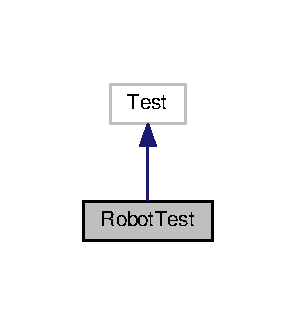
\includegraphics[width=142pt]{class_robot_test__inherit__graph}
\end{center}
\end{figure}


Collaboration diagram for Robot\+Test\+:
\nopagebreak
\begin{figure}[H]
\begin{center}
\leavevmode
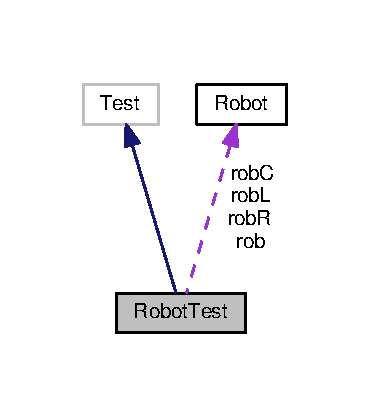
\includegraphics[width=178pt]{class_robot_test__coll__graph}
\end{center}
\end{figure}
\subsection*{Protected Attributes}
\begin{DoxyCompactItemize}
\item 
std\+::string \hyperlink{class_robot_test_ada4ffa3a6eef822a8f5d3c96504decfc}{left} = \char`\"{}left\char`\"{}
\item 
std\+::string \hyperlink{class_robot_test_a95148cd39b86db94058ad7cbd5f4baeb}{right} = \char`\"{}right\char`\"{}
\item 
std\+::string \hyperlink{class_robot_test_a494b9d59a95a0433635069b95f382277}{center} = \char`\"{}center\char`\"{}
\item 
\hyperlink{class_robot}{Robot} \hyperlink{class_robot_test_a2435a71972449d754c6db3bfbe16eb33}{rob}
\item 
\hyperlink{class_robot}{Robot} \hyperlink{class_robot_test_af05d7dded07482862a76de2dde034686}{robL} = \hyperlink{class_robot}{Robot}(\hyperlink{class_robot_test_ada4ffa3a6eef822a8f5d3c96504decfc}{left})
\item 
\hyperlink{class_robot}{Robot} \hyperlink{class_robot_test_a4a293ed153d39518e636bd67839425e3}{robC} = \hyperlink{class_robot}{Robot}(\hyperlink{class_robot_test_a494b9d59a95a0433635069b95f382277}{center})
\item 
\hyperlink{class_robot}{Robot} \hyperlink{class_robot_test_aed2ebf652db21d16a87b9fee909654b9}{robR} = \hyperlink{class_robot}{Robot}(\hyperlink{class_robot_test_a95148cd39b86db94058ad7cbd5f4baeb}{right})
\end{DoxyCompactItemize}


\subsection{Detailed Description}
Class for \hyperlink{class_robot}{Robot} test. 

\subsection{Member Data Documentation}
\index{Robot\+Test@{Robot\+Test}!center@{center}}
\index{center@{center}!Robot\+Test@{Robot\+Test}}
\subsubsection[{\texorpdfstring{center}{center}}]{\setlength{\rightskip}{0pt plus 5cm}std\+::string Robot\+Test\+::center = \char`\"{}center\char`\"{}\hspace{0.3cm}{\ttfamily [protected]}}\hypertarget{class_robot_test_a494b9d59a95a0433635069b95f382277}{}\label{class_robot_test_a494b9d59a95a0433635069b95f382277}
\index{Robot\+Test@{Robot\+Test}!left@{left}}
\index{left@{left}!Robot\+Test@{Robot\+Test}}
\subsubsection[{\texorpdfstring{left}{left}}]{\setlength{\rightskip}{0pt plus 5cm}std\+::string Robot\+Test\+::left = \char`\"{}left\char`\"{}\hspace{0.3cm}{\ttfamily [protected]}}\hypertarget{class_robot_test_ada4ffa3a6eef822a8f5d3c96504decfc}{}\label{class_robot_test_ada4ffa3a6eef822a8f5d3c96504decfc}
\index{Robot\+Test@{Robot\+Test}!right@{right}}
\index{right@{right}!Robot\+Test@{Robot\+Test}}
\subsubsection[{\texorpdfstring{right}{right}}]{\setlength{\rightskip}{0pt plus 5cm}std\+::string Robot\+Test\+::right = \char`\"{}right\char`\"{}\hspace{0.3cm}{\ttfamily [protected]}}\hypertarget{class_robot_test_a95148cd39b86db94058ad7cbd5f4baeb}{}\label{class_robot_test_a95148cd39b86db94058ad7cbd5f4baeb}
\index{Robot\+Test@{Robot\+Test}!rob@{rob}}
\index{rob@{rob}!Robot\+Test@{Robot\+Test}}
\subsubsection[{\texorpdfstring{rob}{rob}}]{\setlength{\rightskip}{0pt plus 5cm}{\bf Robot} Robot\+Test\+::rob\hspace{0.3cm}{\ttfamily [protected]}}\hypertarget{class_robot_test_a2435a71972449d754c6db3bfbe16eb33}{}\label{class_robot_test_a2435a71972449d754c6db3bfbe16eb33}
\index{Robot\+Test@{Robot\+Test}!robC@{robC}}
\index{robC@{robC}!Robot\+Test@{Robot\+Test}}
\subsubsection[{\texorpdfstring{robC}{robC}}]{\setlength{\rightskip}{0pt plus 5cm}{\bf Robot} Robot\+Test\+::robC = {\bf Robot}({\bf center})\hspace{0.3cm}{\ttfamily [protected]}}\hypertarget{class_robot_test_a4a293ed153d39518e636bd67839425e3}{}\label{class_robot_test_a4a293ed153d39518e636bd67839425e3}
\index{Robot\+Test@{Robot\+Test}!robL@{robL}}
\index{robL@{robL}!Robot\+Test@{Robot\+Test}}
\subsubsection[{\texorpdfstring{robL}{robL}}]{\setlength{\rightskip}{0pt plus 5cm}{\bf Robot} Robot\+Test\+::robL = {\bf Robot}({\bf left})\hspace{0.3cm}{\ttfamily [protected]}}\hypertarget{class_robot_test_af05d7dded07482862a76de2dde034686}{}\label{class_robot_test_af05d7dded07482862a76de2dde034686}
\index{Robot\+Test@{Robot\+Test}!robR@{robR}}
\index{robR@{robR}!Robot\+Test@{Robot\+Test}}
\subsubsection[{\texorpdfstring{robR}{robR}}]{\setlength{\rightskip}{0pt plus 5cm}{\bf Robot} Robot\+Test\+::robR = {\bf Robot}({\bf right})\hspace{0.3cm}{\ttfamily [protected]}}\hypertarget{class_robot_test_aed2ebf652db21d16a87b9fee909654b9}{}\label{class_robot_test_aed2ebf652db21d16a87b9fee909654b9}


The documentation for this class was generated from the following file\+:\begin{DoxyCompactItemize}
\item 
test/\hyperlink{_robot_test_8cpp}{Robot\+Test.\+cpp}\end{DoxyCompactItemize}

\hypertarget{class_sensor_fusion_module}{}\section{Sensor\+Fusion\+Module Class Reference}
\label{class_sensor_fusion_module}\index{Sensor\+Fusion\+Module@{Sensor\+Fusion\+Module}}


Class for sensor fusion module.  




{\ttfamily \#include $<$Sensor\+Fusion\+Module.\+hpp$>$}

\subsection*{Public Member Functions}
\begin{DoxyCompactItemize}
\item 
\hyperlink{class_sensor_fusion_module_a197b81625100b2b15d339be6fc15c657}{Sensor\+Fusion\+Module} ()
\begin{DoxyCompactList}\small\item\em Constructor. \end{DoxyCompactList}\item 
\hyperlink{class_sensor_fusion_module_a771099181db2311c47a13b56b93819fb}{$\sim$\+Sensor\+Fusion\+Module} ()\hypertarget{class_sensor_fusion_module_a771099181db2311c47a13b56b93819fb}{}\label{class_sensor_fusion_module_a771099181db2311c47a13b56b93819fb}

\begin{DoxyCompactList}\small\item\em Destroys the object. \end{DoxyCompactList}\item 
void \hyperlink{class_sensor_fusion_module_aa1b418548d329fd79a498edfc476d2b2}{set\+Lidar\+Probabilities} (std\+::vector$<$ float $>$ input)
\begin{DoxyCompactList}\small\item\em Sets the lidar probabilities. \end{DoxyCompactList}\item 
void \hyperlink{class_sensor_fusion_module_af169a79d8e241ba090b13b079d173080}{set\+Image\+Probabilities} (std\+::vector$<$ float $>$ input)
\begin{DoxyCompactList}\small\item\em Sets the image probabilities. \end{DoxyCompactList}\item 
std\+::vector$<$ float $>$ \hyperlink{class_sensor_fusion_module_a13d1756444b5d5e984aed678bed30103}{fuse\+Data} ()
\begin{DoxyCompactList}\small\item\em Fuse the two sensor data. \end{DoxyCompactList}\item 
bool \hyperlink{class_sensor_fusion_module_a8bb7397254888c4204ceeb9540659d4a}{get\+Diagnostic} ()
\begin{DoxyCompactList}\small\item\em Gets the diagnostic. \end{DoxyCompactList}\end{DoxyCompactItemize}


\subsection{Detailed Description}
Class for sensor fusion module. 

Definition at line 24 of file Sensor\+Fusion\+Module.\+hpp.



\subsection{Constructor \& Destructor Documentation}
\index{Sensor\+Fusion\+Module@{Sensor\+Fusion\+Module}!Sensor\+Fusion\+Module@{Sensor\+Fusion\+Module}}
\index{Sensor\+Fusion\+Module@{Sensor\+Fusion\+Module}!Sensor\+Fusion\+Module@{Sensor\+Fusion\+Module}}
\subsubsection[{\texorpdfstring{Sensor\+Fusion\+Module()}{SensorFusionModule()}}]{\setlength{\rightskip}{0pt plus 5cm}Sensor\+Fusion\+Module\+::\+Sensor\+Fusion\+Module (
\begin{DoxyParamCaption}
{}
\end{DoxyParamCaption}
)}\hypertarget{class_sensor_fusion_module_a197b81625100b2b15d339be6fc15c657}{}\label{class_sensor_fusion_module_a197b81625100b2b15d339be6fc15c657}


Constructor. 

Constructs the object. 

Definition at line 21 of file Sensor\+Fusion\+Module.\+cpp.



\subsection{Member Function Documentation}
\index{Sensor\+Fusion\+Module@{Sensor\+Fusion\+Module}!fuse\+Data@{fuse\+Data}}
\index{fuse\+Data@{fuse\+Data}!Sensor\+Fusion\+Module@{Sensor\+Fusion\+Module}}
\subsubsection[{\texorpdfstring{fuse\+Data()}{fuseData()}}]{\setlength{\rightskip}{0pt plus 5cm}std\+::vector$<$ float $>$ Sensor\+Fusion\+Module\+::fuse\+Data (
\begin{DoxyParamCaption}
{}
\end{DoxyParamCaption}
)}\hypertarget{class_sensor_fusion_module_a13d1756444b5d5e984aed678bed30103}{}\label{class_sensor_fusion_module_a13d1756444b5d5e984aed678bed30103}


Fuse the two sensor data. 

\begin{DoxyReturn}{Returns}
Fused sensor probabilities 
\end{DoxyReturn}


Definition at line 53 of file Sensor\+Fusion\+Module.\+cpp.

\index{Sensor\+Fusion\+Module@{Sensor\+Fusion\+Module}!get\+Diagnostic@{get\+Diagnostic}}
\index{get\+Diagnostic@{get\+Diagnostic}!Sensor\+Fusion\+Module@{Sensor\+Fusion\+Module}}
\subsubsection[{\texorpdfstring{get\+Diagnostic()}{getDiagnostic()}}]{\setlength{\rightskip}{0pt plus 5cm}bool Sensor\+Fusion\+Module\+::get\+Diagnostic (
\begin{DoxyParamCaption}
{}
\end{DoxyParamCaption}
)}\hypertarget{class_sensor_fusion_module_a8bb7397254888c4204ceeb9540659d4a}{}\label{class_sensor_fusion_module_a8bb7397254888c4204ceeb9540659d4a}


Gets the diagnostic. 

\begin{DoxyReturn}{Returns}
The diagnostic truth value. 
\end{DoxyReturn}


Definition at line 72 of file Sensor\+Fusion\+Module.\+cpp.

\index{Sensor\+Fusion\+Module@{Sensor\+Fusion\+Module}!set\+Image\+Probabilities@{set\+Image\+Probabilities}}
\index{set\+Image\+Probabilities@{set\+Image\+Probabilities}!Sensor\+Fusion\+Module@{Sensor\+Fusion\+Module}}
\subsubsection[{\texorpdfstring{set\+Image\+Probabilities(std\+::vector$<$ float $>$ input)}{setImageProbabilities(std::vector< float > input)}}]{\setlength{\rightskip}{0pt plus 5cm}void Sensor\+Fusion\+Module\+::set\+Image\+Probabilities (
\begin{DoxyParamCaption}
\item[{std\+::vector$<$ float $>$}]{input}
\end{DoxyParamCaption}
)}\hypertarget{class_sensor_fusion_module_af169a79d8e241ba090b13b079d173080}{}\label{class_sensor_fusion_module_af169a79d8e241ba090b13b079d173080}


Sets the image probabilities. 


\begin{DoxyParams}[1]{Parameters}
\mbox{\tt in}  & {\em input} & The input \\
\hline
\end{DoxyParams}


Definition at line 44 of file Sensor\+Fusion\+Module.\+cpp.

\index{Sensor\+Fusion\+Module@{Sensor\+Fusion\+Module}!set\+Lidar\+Probabilities@{set\+Lidar\+Probabilities}}
\index{set\+Lidar\+Probabilities@{set\+Lidar\+Probabilities}!Sensor\+Fusion\+Module@{Sensor\+Fusion\+Module}}
\subsubsection[{\texorpdfstring{set\+Lidar\+Probabilities(std\+::vector$<$ float $>$ input)}{setLidarProbabilities(std::vector< float > input)}}]{\setlength{\rightskip}{0pt plus 5cm}void Sensor\+Fusion\+Module\+::set\+Lidar\+Probabilities (
\begin{DoxyParamCaption}
\item[{std\+::vector$<$ float $>$}]{input}
\end{DoxyParamCaption}
)}\hypertarget{class_sensor_fusion_module_aa1b418548d329fd79a498edfc476d2b2}{}\label{class_sensor_fusion_module_aa1b418548d329fd79a498edfc476d2b2}


Sets the lidar probabilities. 

Sets the heading direction.


\begin{DoxyParams}[1]{Parameters}
\mbox{\tt in}  & {\em input} & The input \\
\hline
\end{DoxyParams}


Definition at line 35 of file Sensor\+Fusion\+Module.\+cpp.



The documentation for this class was generated from the following files\+:\begin{DoxyCompactItemize}
\item 
include/\hyperlink{_sensor_fusion_module_8hpp}{Sensor\+Fusion\+Module.\+hpp}\item 
app/\hyperlink{_sensor_fusion_module_8cpp}{Sensor\+Fusion\+Module.\+cpp}\end{DoxyCompactItemize}

\hypertarget{class_sensor_fusion_test}{}\section{Sensor\+Fusion\+Test Class Reference}
\label{class_sensor_fusion_test}\index{Sensor\+Fusion\+Test@{Sensor\+Fusion\+Test}}


Class for sensor fusion test.  




Inheritance diagram for Sensor\+Fusion\+Test\+:
\nopagebreak
\begin{figure}[H]
\begin{center}
\leavevmode
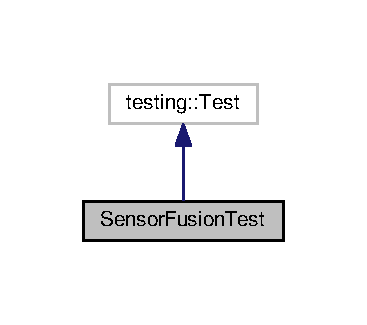
\includegraphics[width=176pt]{class_sensor_fusion_test__inherit__graph}
\end{center}
\end{figure}


Collaboration diagram for Sensor\+Fusion\+Test\+:
\nopagebreak
\begin{figure}[H]
\begin{center}
\leavevmode
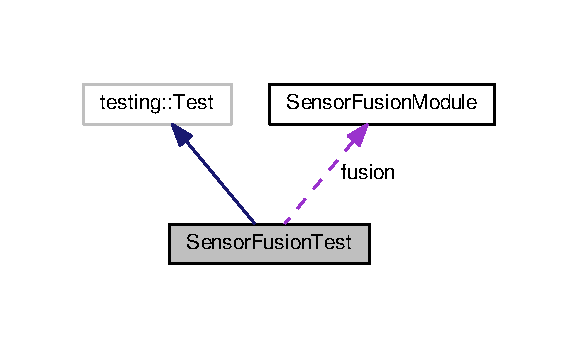
\includegraphics[width=278pt]{class_sensor_fusion_test__coll__graph}
\end{center}
\end{figure}
\subsection*{Protected Attributes}
\begin{DoxyCompactItemize}
\item 
\hyperlink{class_sensor_fusion_module}{Sensor\+Fusion\+Module} \hyperlink{class_sensor_fusion_test_a2f23e29ade2dcdec5510cc2b893c9cc7}{fusion}
\end{DoxyCompactItemize}


\subsection{Detailed Description}
Class for sensor fusion test. 

\subsection{Member Data Documentation}
\index{Sensor\+Fusion\+Test@{Sensor\+Fusion\+Test}!fusion@{fusion}}
\index{fusion@{fusion}!Sensor\+Fusion\+Test@{Sensor\+Fusion\+Test}}
\subsubsection[{\texorpdfstring{fusion}{fusion}}]{\setlength{\rightskip}{0pt plus 5cm}{\bf Sensor\+Fusion\+Module} Sensor\+Fusion\+Test\+::fusion\hspace{0.3cm}{\ttfamily [protected]}}\hypertarget{class_sensor_fusion_test_a2f23e29ade2dcdec5510cc2b893c9cc7}{}\label{class_sensor_fusion_test_a2f23e29ade2dcdec5510cc2b893c9cc7}


The documentation for this class was generated from the following file\+:\begin{DoxyCompactItemize}
\item 
test/\hyperlink{_sensor_fusion_test_8cpp}{Sensor\+Fusion\+Test.\+cpp}\end{DoxyCompactItemize}

\chapter{File Documentation}
\hypertarget{_8ycm__extra__conf_8py}{}\section{.ycm\+\_\+extra\+\_\+conf.\+py File Reference}
\label{_8ycm__extra__conf_8py}\index{.\+ycm\+\_\+extra\+\_\+conf.\+py@{.\+ycm\+\_\+extra\+\_\+conf.\+py}}
\subsection*{Functions}
\begin{DoxyCompactItemize}
\item 
def \hyperlink{_8ycm__extra__conf_8py_aab283cdb607efa6a1a7aaa3f089c63f1}{Directory\+Of\+This\+Script} ()
\item 
def \hyperlink{_8ycm__extra__conf_8py_aa20d30f8cc08fc0ab076b4cf458e0d3d}{Make\+Relative\+Paths\+In\+Flags\+Absolute} (\hyperlink{_8ycm__extra__conf_8py_abd73d8e4551f1a637280b3876d1ae2e3}{flags}, working\+\_\+directory)
\item 
def \hyperlink{_8ycm__extra__conf_8py_a6bb59f541be0dcbde53eba606d48ddf8}{Is\+Header\+File} (filename)
\item 
def \hyperlink{_8ycm__extra__conf_8py_a42a14573593ce75cd6e385a85326111f}{Get\+Compilation\+Info\+For\+File} (filename)
\item 
def \hyperlink{_8ycm__extra__conf_8py_a51f8bcdc9a3b791e6a88d798e6c786b3}{Flags\+For\+File} (filename, kwargs)
\end{DoxyCompactItemize}
\subsection*{Variables}
\begin{DoxyCompactItemize}
\item 
list \hyperlink{_8ycm__extra__conf_8py_abd73d8e4551f1a637280b3876d1ae2e3}{flags}
\item 
string \hyperlink{_8ycm__extra__conf_8py_a6a4d7e96c7bc9093b406af626b7936a2}{compilation\+\_\+database\+\_\+folder} = \textquotesingle{}\textquotesingle{}
\item 
\hyperlink{_8ycm__extra__conf_8py_a64dbaa3229ec575b68ec333442e10cee}{database} = ycm\+\_\+core.\+Compilation\+Database( \hyperlink{_8ycm__extra__conf_8py_a6a4d7e96c7bc9093b406af626b7936a2}{compilation\+\_\+database\+\_\+folder} )
\item 
list \hyperlink{_8ycm__extra__conf_8py_a47014996e1e517071cd0412a22adb123}{S\+O\+U\+R\+C\+E\+\_\+\+E\+X\+T\+E\+N\+S\+I\+O\+NS} = \mbox{[} \textquotesingle{}.C\textquotesingle{}, \textquotesingle{}.cpp\textquotesingle{}, \textquotesingle{}.cxx\textquotesingle{}, \textquotesingle{}.cc\textquotesingle{}, \textquotesingle{}.c\textquotesingle{}, \textquotesingle{}.m\textquotesingle{}, \textquotesingle{}.mm\textquotesingle{} \mbox{]}
\end{DoxyCompactItemize}


\subsection{Function Documentation}
\index{.\+ycm\+\_\+extra\+\_\+conf.\+py@{.\+ycm\+\_\+extra\+\_\+conf.\+py}!Directory\+Of\+This\+Script@{Directory\+Of\+This\+Script}}
\index{Directory\+Of\+This\+Script@{Directory\+Of\+This\+Script}!.\+ycm\+\_\+extra\+\_\+conf.\+py@{.\+ycm\+\_\+extra\+\_\+conf.\+py}}
\subsubsection[{\texorpdfstring{Directory\+Of\+This\+Script()}{DirectoryOfThisScript()}}]{\setlength{\rightskip}{0pt plus 5cm}def Directory\+Of\+This\+Script (
\begin{DoxyParamCaption}
{}
\end{DoxyParamCaption}
)}\hypertarget{_8ycm__extra__conf_8py_aab283cdb607efa6a1a7aaa3f089c63f1}{}\label{_8ycm__extra__conf_8py_aab283cdb607efa6a1a7aaa3f089c63f1}
\index{.\+ycm\+\_\+extra\+\_\+conf.\+py@{.\+ycm\+\_\+extra\+\_\+conf.\+py}!Flags\+For\+File@{Flags\+For\+File}}
\index{Flags\+For\+File@{Flags\+For\+File}!.\+ycm\+\_\+extra\+\_\+conf.\+py@{.\+ycm\+\_\+extra\+\_\+conf.\+py}}
\subsubsection[{\texorpdfstring{Flags\+For\+File(filename, kwargs)}{FlagsForFile(filename, kwargs)}}]{\setlength{\rightskip}{0pt plus 5cm}def Flags\+For\+File (
\begin{DoxyParamCaption}
\item[{}]{filename, }
\item[{}]{kwargs}
\end{DoxyParamCaption}
)}\hypertarget{_8ycm__extra__conf_8py_a51f8bcdc9a3b791e6a88d798e6c786b3}{}\label{_8ycm__extra__conf_8py_a51f8bcdc9a3b791e6a88d798e6c786b3}
\index{.\+ycm\+\_\+extra\+\_\+conf.\+py@{.\+ycm\+\_\+extra\+\_\+conf.\+py}!Get\+Compilation\+Info\+For\+File@{Get\+Compilation\+Info\+For\+File}}
\index{Get\+Compilation\+Info\+For\+File@{Get\+Compilation\+Info\+For\+File}!.\+ycm\+\_\+extra\+\_\+conf.\+py@{.\+ycm\+\_\+extra\+\_\+conf.\+py}}
\subsubsection[{\texorpdfstring{Get\+Compilation\+Info\+For\+File(filename)}{GetCompilationInfoForFile(filename)}}]{\setlength{\rightskip}{0pt plus 5cm}def Get\+Compilation\+Info\+For\+File (
\begin{DoxyParamCaption}
\item[{}]{filename}
\end{DoxyParamCaption}
)}\hypertarget{_8ycm__extra__conf_8py_a42a14573593ce75cd6e385a85326111f}{}\label{_8ycm__extra__conf_8py_a42a14573593ce75cd6e385a85326111f}
\index{.\+ycm\+\_\+extra\+\_\+conf.\+py@{.\+ycm\+\_\+extra\+\_\+conf.\+py}!Is\+Header\+File@{Is\+Header\+File}}
\index{Is\+Header\+File@{Is\+Header\+File}!.\+ycm\+\_\+extra\+\_\+conf.\+py@{.\+ycm\+\_\+extra\+\_\+conf.\+py}}
\subsubsection[{\texorpdfstring{Is\+Header\+File(filename)}{IsHeaderFile(filename)}}]{\setlength{\rightskip}{0pt plus 5cm}def Is\+Header\+File (
\begin{DoxyParamCaption}
\item[{}]{filename}
\end{DoxyParamCaption}
)}\hypertarget{_8ycm__extra__conf_8py_a6bb59f541be0dcbde53eba606d48ddf8}{}\label{_8ycm__extra__conf_8py_a6bb59f541be0dcbde53eba606d48ddf8}
\index{.\+ycm\+\_\+extra\+\_\+conf.\+py@{.\+ycm\+\_\+extra\+\_\+conf.\+py}!Make\+Relative\+Paths\+In\+Flags\+Absolute@{Make\+Relative\+Paths\+In\+Flags\+Absolute}}
\index{Make\+Relative\+Paths\+In\+Flags\+Absolute@{Make\+Relative\+Paths\+In\+Flags\+Absolute}!.\+ycm\+\_\+extra\+\_\+conf.\+py@{.\+ycm\+\_\+extra\+\_\+conf.\+py}}
\subsubsection[{\texorpdfstring{Make\+Relative\+Paths\+In\+Flags\+Absolute(flags, working\+\_\+directory)}{MakeRelativePathsInFlagsAbsolute(flags, working_directory)}}]{\setlength{\rightskip}{0pt plus 5cm}def Make\+Relative\+Paths\+In\+Flags\+Absolute (
\begin{DoxyParamCaption}
\item[{}]{flags, }
\item[{}]{working\+\_\+directory}
\end{DoxyParamCaption}
)}\hypertarget{_8ycm__extra__conf_8py_aa20d30f8cc08fc0ab076b4cf458e0d3d}{}\label{_8ycm__extra__conf_8py_aa20d30f8cc08fc0ab076b4cf458e0d3d}


\subsection{Variable Documentation}
\index{.\+ycm\+\_\+extra\+\_\+conf.\+py@{.\+ycm\+\_\+extra\+\_\+conf.\+py}!compilation\+\_\+database\+\_\+folder@{compilation\+\_\+database\+\_\+folder}}
\index{compilation\+\_\+database\+\_\+folder@{compilation\+\_\+database\+\_\+folder}!.\+ycm\+\_\+extra\+\_\+conf.\+py@{.\+ycm\+\_\+extra\+\_\+conf.\+py}}
\subsubsection[{\texorpdfstring{compilation\+\_\+database\+\_\+folder}{compilation_database_folder}}]{\setlength{\rightskip}{0pt plus 5cm}string compilation\+\_\+database\+\_\+folder = \textquotesingle{}\textquotesingle{}}\hypertarget{_8ycm__extra__conf_8py_a6a4d7e96c7bc9093b406af626b7936a2}{}\label{_8ycm__extra__conf_8py_a6a4d7e96c7bc9093b406af626b7936a2}
\index{.\+ycm\+\_\+extra\+\_\+conf.\+py@{.\+ycm\+\_\+extra\+\_\+conf.\+py}!database@{database}}
\index{database@{database}!.\+ycm\+\_\+extra\+\_\+conf.\+py@{.\+ycm\+\_\+extra\+\_\+conf.\+py}}
\subsubsection[{\texorpdfstring{database}{database}}]{\setlength{\rightskip}{0pt plus 5cm}database = ycm\+\_\+core.\+Compilation\+Database( {\bf compilation\+\_\+database\+\_\+folder} )}\hypertarget{_8ycm__extra__conf_8py_a64dbaa3229ec575b68ec333442e10cee}{}\label{_8ycm__extra__conf_8py_a64dbaa3229ec575b68ec333442e10cee}
\index{.\+ycm\+\_\+extra\+\_\+conf.\+py@{.\+ycm\+\_\+extra\+\_\+conf.\+py}!flags@{flags}}
\index{flags@{flags}!.\+ycm\+\_\+extra\+\_\+conf.\+py@{.\+ycm\+\_\+extra\+\_\+conf.\+py}}
\subsubsection[{\texorpdfstring{flags}{flags}}]{\setlength{\rightskip}{0pt plus 5cm}list flags}\hypertarget{_8ycm__extra__conf_8py_abd73d8e4551f1a637280b3876d1ae2e3}{}\label{_8ycm__extra__conf_8py_abd73d8e4551f1a637280b3876d1ae2e3}
{\bfseries Initial value\+:}
\begin{DoxyCode}
1 = [
2     \textcolor{stringliteral}{'-x'},
3     \textcolor{stringliteral}{'c++'},
4     \textcolor{stringliteral}{'-DGTEST\_HAS\_PTHREAD=1'},
5     \textcolor{stringliteral}{'-I/Users/david/code/scratch/cpp/include'},
6     \textcolor{stringliteral}{'-I/Users/david/code/scratch/cpp/test/../vendor/googletest/googletest/include'},
7     \textcolor{stringliteral}{'-I/Users/david/code/scratch/cpp/vendor/boost'},
8     \textcolor{stringliteral}{'-I/Users/david/code/scratch/cpp/vendor/googletest/googletest'},
9     \textcolor{stringliteral}{'-I/Users/david/code/scratch/cpp/vendor/googletest/googletest/include'},
10     \textcolor{stringliteral}{'-Wall'},
11     \textcolor{stringliteral}{'-Wextra'},
12     \textcolor{stringliteral}{'-Wpedantic'},
13     \textcolor{stringliteral}{'-std=c++14'},
14 ]
\end{DoxyCode}
\index{.\+ycm\+\_\+extra\+\_\+conf.\+py@{.\+ycm\+\_\+extra\+\_\+conf.\+py}!S\+O\+U\+R\+C\+E\+\_\+\+E\+X\+T\+E\+N\+S\+I\+O\+NS@{S\+O\+U\+R\+C\+E\+\_\+\+E\+X\+T\+E\+N\+S\+I\+O\+NS}}
\index{S\+O\+U\+R\+C\+E\+\_\+\+E\+X\+T\+E\+N\+S\+I\+O\+NS@{S\+O\+U\+R\+C\+E\+\_\+\+E\+X\+T\+E\+N\+S\+I\+O\+NS}!.\+ycm\+\_\+extra\+\_\+conf.\+py@{.\+ycm\+\_\+extra\+\_\+conf.\+py}}
\subsubsection[{\texorpdfstring{S\+O\+U\+R\+C\+E\+\_\+\+E\+X\+T\+E\+N\+S\+I\+O\+NS}{SOURCE_EXTENSIONS}}]{\setlength{\rightskip}{0pt plus 5cm}list S\+O\+U\+R\+C\+E\+\_\+\+E\+X\+T\+E\+N\+S\+I\+O\+NS = \mbox{[} \textquotesingle{}.C\textquotesingle{}, \textquotesingle{}.cpp\textquotesingle{}, \textquotesingle{}.cxx\textquotesingle{}, \textquotesingle{}.cc\textquotesingle{}, \textquotesingle{}.c\textquotesingle{}, \textquotesingle{}.m\textquotesingle{}, \textquotesingle{}.mm\textquotesingle{} \mbox{]}}\hypertarget{_8ycm__extra__conf_8py_a47014996e1e517071cd0412a22adb123}{}\label{_8ycm__extra__conf_8py_a47014996e1e517071cd0412a22adb123}

\hypertarget{_camera_module_8cpp}{}\section{app/\+Camera\+Module.cpp File Reference}
\label{_camera_module_8cpp}\index{app/\+Camera\+Module.\+cpp@{app/\+Camera\+Module.\+cpp}}


E\+N\+P\+M808X, Midsemester project.  


{\ttfamily \#include $<$vector$>$}\\*
{\ttfamily \#include \char`\"{}Camera\+Module.\+hpp\char`\"{}}\\*
Include dependency graph for Camera\+Module.\+cpp\+:
\nopagebreak
\begin{figure}[H]
\begin{center}
\leavevmode
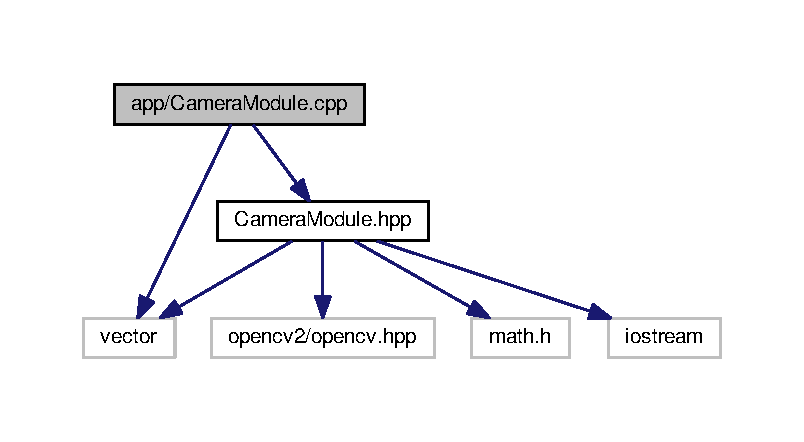
\includegraphics[width=350pt]{_camera_module_8cpp__incl}
\end{center}
\end{figure}


\subsection{Detailed Description}
E\+N\+P\+M808X, Midsemester project. 

\begin{DoxyAuthor}{Author}
Karan Vivek Bhargava 
\end{DoxyAuthor}
\begin{DoxyCopyright}{Copyright}
M\+IT License
\end{DoxyCopyright}
\hypertarget{_robot_test_8cpp_DESCRIPTION}{}\subsection{D\+E\+S\+C\+R\+I\+P\+T\+I\+ON}\label{_robot_test_8cpp_DESCRIPTION}
This program is controlling a robot\textquotesingle{}s heading direction using sensor fusion. 
\hypertarget{_lidar_module_8cpp}{}\section{app/\+Lidar\+Module.cpp File Reference}
\label{_lidar_module_8cpp}\index{app/\+Lidar\+Module.\+cpp@{app/\+Lidar\+Module.\+cpp}}


E\+N\+P\+M808X, Midsemester project.  


{\ttfamily \#include $<$vector$>$}\\*
{\ttfamily \#include $<$string$>$}\\*
{\ttfamily \#include \char`\"{}Lidar\+Module.\+hpp\char`\"{}}\\*
Include dependency graph for Lidar\+Module.\+cpp\+:
\nopagebreak
\begin{figure}[H]
\begin{center}
\leavevmode
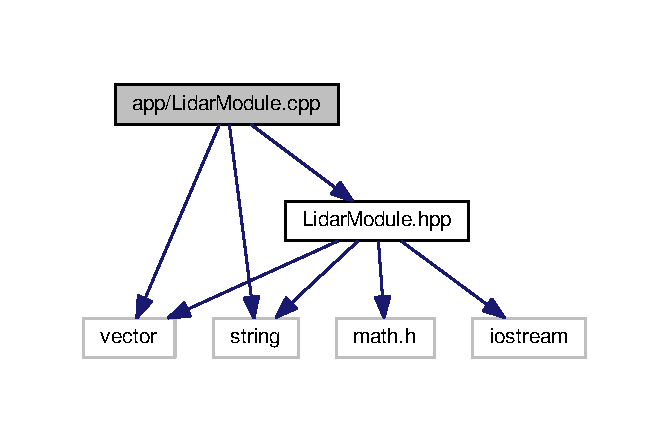
\includegraphics[width=321pt]{_lidar_module_8cpp__incl}
\end{center}
\end{figure}


\subsection{Detailed Description}
E\+N\+P\+M808X, Midsemester project. 

\begin{DoxyAuthor}{Author}
Karan Vivek Bhargava 
\end{DoxyAuthor}
\begin{DoxyCopyright}{Copyright}
M\+IT License
\end{DoxyCopyright}
\hypertarget{_path_planning_test_8cpp_DESCRIPTION}{}\subsection{D\+E\+S\+C\+R\+I\+P\+T\+I\+ON}\label{_path_planning_test_8cpp_DESCRIPTION}
This program is controlling a robot\textquotesingle{}s heading direction using sensor fusion. 
\hypertarget{app_2main_8cpp}{}\section{app/main.cpp File Reference}
\label{app_2main_8cpp}\index{app/main.\+cpp@{app/main.\+cpp}}
{\ttfamily \#include $<$Robot.\+hpp$>$}\\*
{\ttfamily \#include $<$string$>$}\\*
Include dependency graph for main.\+cpp\+:
\nopagebreak
\begin{figure}[H]
\begin{center}
\leavevmode
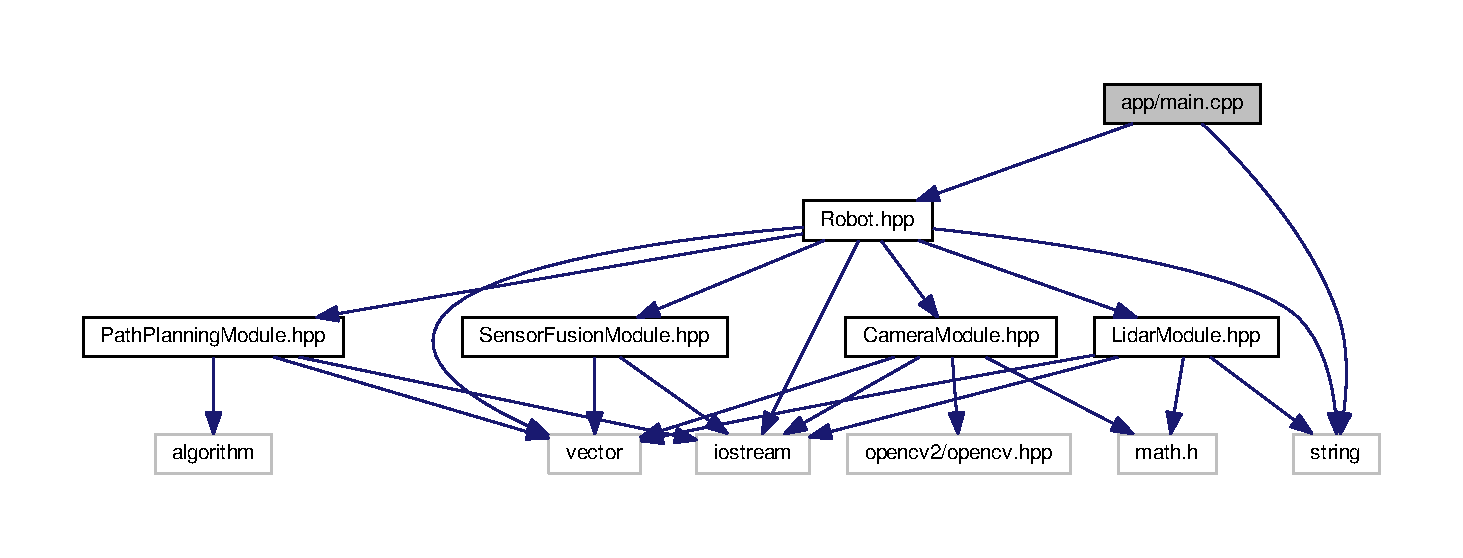
\includegraphics[width=350pt]{app_2main_8cpp__incl}
\end{center}
\end{figure}
\subsection*{Functions}
\begin{DoxyCompactItemize}
\item 
int \hyperlink{app_2main_8cpp_a0ddf1224851353fc92bfbff6f499fa97}{main} (int argc, char $\ast$argv\mbox{[}$\,$\mbox{]})
\begin{DoxyCompactList}\small\item\em main function \end{DoxyCompactList}\end{DoxyCompactItemize}


\subsection{Function Documentation}
\index{app/main.\+cpp@{app/main.\+cpp}!main@{main}}
\index{main@{main}!app/main.\+cpp@{app/main.\+cpp}}
\subsubsection[{\texorpdfstring{main(int argc, char $\ast$argv[])}{main(int argc, char *argv[])}}]{\setlength{\rightskip}{0pt plus 5cm}int main (
\begin{DoxyParamCaption}
\item[{int}]{argc, }
\item[{char $\ast$}]{argv\mbox{[}$\,$\mbox{]}}
\end{DoxyParamCaption}
)}\hypertarget{app_2main_8cpp_a0ddf1224851353fc92bfbff6f499fa97}{}\label{app_2main_8cpp_a0ddf1224851353fc92bfbff6f499fa97}


main function 

\begin{DoxyReturn}{Returns}
nothing 
\end{DoxyReturn}

\hypertarget{test_2main_8cpp}{}\section{test/main.cpp File Reference}
\label{test_2main_8cpp}\index{test/main.\+cpp@{test/main.\+cpp}}
{\ttfamily \#include $<$gtest/gtest.\+h$>$}\\*
Include dependency graph for main.\+cpp\+:
\nopagebreak
\begin{figure}[H]
\begin{center}
\leavevmode
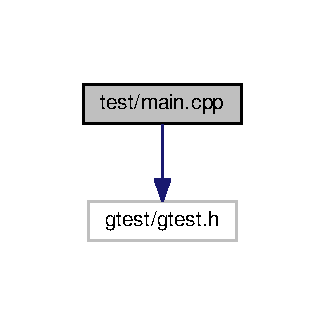
\includegraphics[width=156pt]{test_2main_8cpp__incl}
\end{center}
\end{figure}
\subsection*{Functions}
\begin{DoxyCompactItemize}
\item 
int \hyperlink{test_2main_8cpp_a3c04138a5bfe5d72780bb7e82a18e627}{main} (int argc, char $\ast$$\ast$argv)
\begin{DoxyCompactList}\small\item\em This is the main function for testing. \end{DoxyCompactList}\end{DoxyCompactItemize}


\subsection{Function Documentation}
\index{test/main.\+cpp@{test/main.\+cpp}!main@{main}}
\index{main@{main}!test/main.\+cpp@{test/main.\+cpp}}
\subsubsection[{\texorpdfstring{main(int argc, char $\ast$$\ast$argv)}{main(int argc, char **argv)}}]{\setlength{\rightskip}{0pt plus 5cm}int main (
\begin{DoxyParamCaption}
\item[{int}]{argc, }
\item[{char $\ast$$\ast$}]{argv}
\end{DoxyParamCaption}
)}\hypertarget{test_2main_8cpp_a3c04138a5bfe5d72780bb7e82a18e627}{}\label{test_2main_8cpp_a3c04138a5bfe5d72780bb7e82a18e627}


This is the main function for testing. 


\begin{DoxyParams}[1]{Parameters}
\mbox{\tt in}  & {\em argc} & The argc \\
\hline
 & {\em argv} & The argv\\
\hline
\end{DoxyParams}
\begin{DoxyReturn}{Returns}
nothing, just runs all the tests 
\end{DoxyReturn}

\hypertarget{_path_planning_module_8cpp}{}\section{app/\+Path\+Planning\+Module.cpp File Reference}
\label{_path_planning_module_8cpp}\index{app/\+Path\+Planning\+Module.\+cpp@{app/\+Path\+Planning\+Module.\+cpp}}


E\+N\+P\+M808X, Midsemester project.  


{\ttfamily \#include $<$algorithm$>$}\\*
{\ttfamily \#include $<$vector$>$}\\*
{\ttfamily \#include \char`\"{}Path\+Planning\+Module.\+hpp\char`\"{}}\\*
Include dependency graph for Path\+Planning\+Module.\+cpp\+:
\nopagebreak
\begin{figure}[H]
\begin{center}
\leavevmode
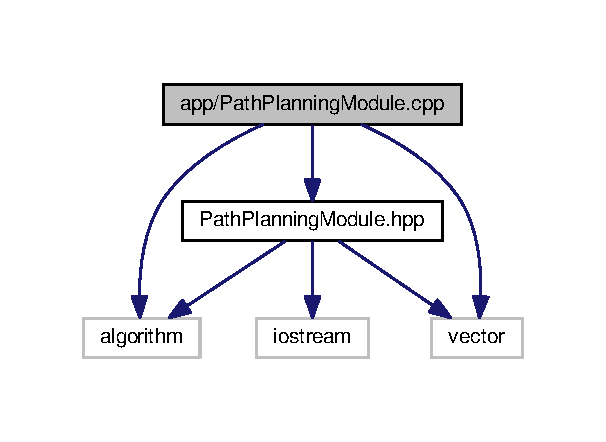
\includegraphics[width=291pt]{_path_planning_module_8cpp__incl}
\end{center}
\end{figure}


\subsection{Detailed Description}
E\+N\+P\+M808X, Midsemester project. 

\begin{DoxyAuthor}{Author}
Karan Vivek Bhargava 
\end{DoxyAuthor}
\begin{DoxyCopyright}{Copyright}
M\+IT License
\end{DoxyCopyright}
\hypertarget{_robot_test_8cpp_DESCRIPTION}{}\subsection{D\+E\+S\+C\+R\+I\+P\+T\+I\+ON}\label{_robot_test_8cpp_DESCRIPTION}
This program is controlling a robot\textquotesingle{}s heading direction using sensor fusion. 
\hypertarget{_robot_8cpp}{}\section{app/\+Robot.cpp File Reference}
\label{_robot_8cpp}\index{app/\+Robot.\+cpp@{app/\+Robot.\+cpp}}


E\+N\+P\+M808X, Midsemester project.  


{\ttfamily \#include $<$Robot.\+hpp$>$}\\*
Include dependency graph for Robot.\+cpp\+:
\nopagebreak
\begin{figure}[H]
\begin{center}
\leavevmode
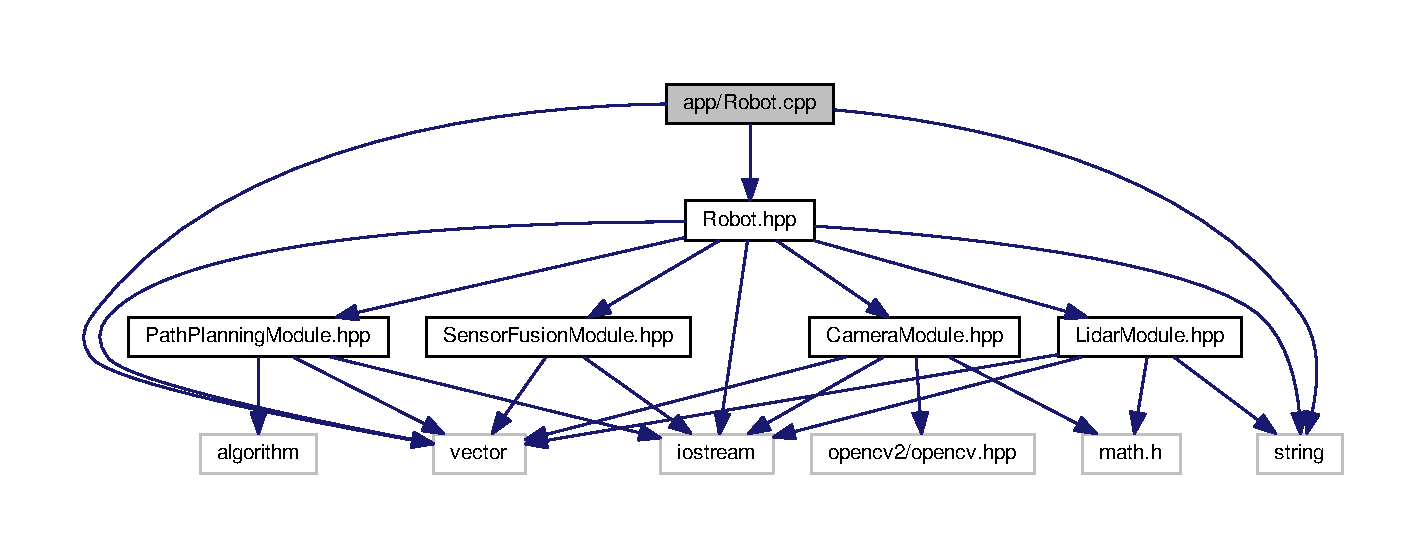
\includegraphics[width=350pt]{_robot_8cpp__incl}
\end{center}
\end{figure}


\subsection{Detailed Description}
E\+N\+P\+M808X, Midsemester project. 

\begin{DoxyAuthor}{Author}
Karan Vivek Bhargava 
\end{DoxyAuthor}
\begin{DoxyCopyright}{Copyright}
M\+IT License
\end{DoxyCopyright}
\hypertarget{_path_planning_test_8cpp_DESCRIPTION}{}\subsection{D\+E\+S\+C\+R\+I\+P\+T\+I\+ON}\label{_path_planning_test_8cpp_DESCRIPTION}
This program is controlling a robot\textquotesingle{}s heading direction using sensor fusion. 
\hypertarget{_sensor_fusion_module_8cpp}{}\section{app/\+Sensor\+Fusion\+Module.cpp File Reference}
\label{_sensor_fusion_module_8cpp}\index{app/\+Sensor\+Fusion\+Module.\+cpp@{app/\+Sensor\+Fusion\+Module.\+cpp}}


E\+N\+P\+M808X, Midsemester project.  


{\ttfamily \#include $<$vector$>$}\\*
{\ttfamily \#include \char`\"{}Sensor\+Fusion\+Module.\+hpp\char`\"{}}\\*
Include dependency graph for Sensor\+Fusion\+Module.\+cpp\+:
\nopagebreak
\begin{figure}[H]
\begin{center}
\leavevmode
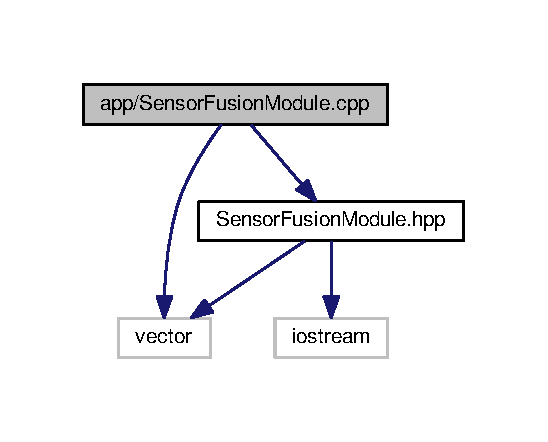
\includegraphics[width=263pt]{_sensor_fusion_module_8cpp__incl}
\end{center}
\end{figure}


\subsection{Detailed Description}
E\+N\+P\+M808X, Midsemester project. 

\begin{DoxyAuthor}{Author}
Karan Vivek Bhargava 
\end{DoxyAuthor}
\begin{DoxyCopyright}{Copyright}
M\+IT License
\end{DoxyCopyright}
\hypertarget{_path_planning_test_8cpp_DESCRIPTION}{}\subsection{D\+E\+S\+C\+R\+I\+P\+T\+I\+ON}\label{_path_planning_test_8cpp_DESCRIPTION}
This program is controlling a robot\textquotesingle{}s heading direction using sensor fusion. 
\hypertarget{_camera_module_8hpp}{}\section{include/\+Camera\+Module.hpp File Reference}
\label{_camera_module_8hpp}\index{include/\+Camera\+Module.\+hpp@{include/\+Camera\+Module.\+hpp}}


E\+N\+P\+M808X, Midsemester project.  


{\ttfamily \#include $<$opencv2/opencv.\+hpp$>$}\\*
{\ttfamily \#include $<$math.\+h$>$}\\*
{\ttfamily \#include $<$iostream$>$}\\*
{\ttfamily \#include $<$vector$>$}\\*
Include dependency graph for Camera\+Module.\+hpp\+:
\nopagebreak
\begin{figure}[H]
\begin{center}
\leavevmode
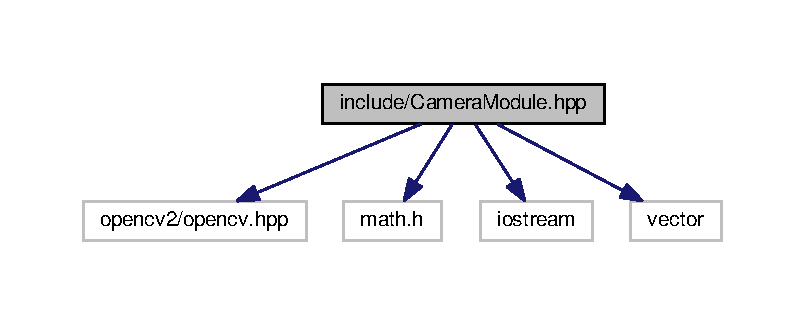
\includegraphics[width=350pt]{_camera_module_8hpp__incl}
\end{center}
\end{figure}
This graph shows which files directly or indirectly include this file\+:
\nopagebreak
\begin{figure}[H]
\begin{center}
\leavevmode
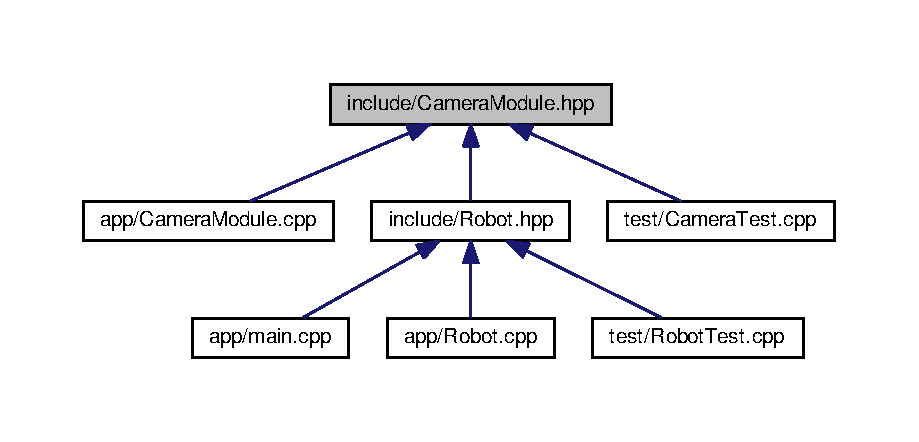
\includegraphics[width=350pt]{_camera_module_8hpp__dep__incl}
\end{center}
\end{figure}
\subsection*{Classes}
\begin{DoxyCompactItemize}
\item 
class \hyperlink{class_camera_module}{Camera\+Module}
\begin{DoxyCompactList}\small\item\em Class for camera module. \end{DoxyCompactList}\end{DoxyCompactItemize}
\subsection*{Macros}
\begin{DoxyCompactItemize}
\item 
\#define {\bfseries PI}~3.\+14159265\hypertarget{_camera_module_8hpp_a598a3330b3c21701223ee0ca14316eca}{}\label{_camera_module_8hpp_a598a3330b3c21701223ee0ca14316eca}

\end{DoxyCompactItemize}


\subsection{Detailed Description}
E\+N\+P\+M808X, Midsemester project. 

\begin{DoxyAuthor}{Author}
Karan Vivek Bhargava 
\end{DoxyAuthor}
\begin{DoxyCopyright}{Copyright}
M\+IT License
\end{DoxyCopyright}
\hypertarget{_path_planning_test_8cpp_DESCRIPTION}{}\subsection{D\+E\+S\+C\+R\+I\+P\+T\+I\+ON}\label{_path_planning_test_8cpp_DESCRIPTION}
This program is controlling a robot\textquotesingle{}s heading direction using sensor fusion. 
\hypertarget{_lidar_module_8hpp}{}\section{include/\+Lidar\+Module.hpp File Reference}
\label{_lidar_module_8hpp}\index{include/\+Lidar\+Module.\+hpp@{include/\+Lidar\+Module.\+hpp}}


E\+N\+P\+M808X, Midsemester project.  


{\ttfamily \#include $<$math.\+h$>$}\\*
{\ttfamily \#include $<$iostream$>$}\\*
{\ttfamily \#include $<$vector$>$}\\*
{\ttfamily \#include $<$string$>$}\\*
Include dependency graph for Lidar\+Module.\+hpp\+:
\nopagebreak
\begin{figure}[H]
\begin{center}
\leavevmode
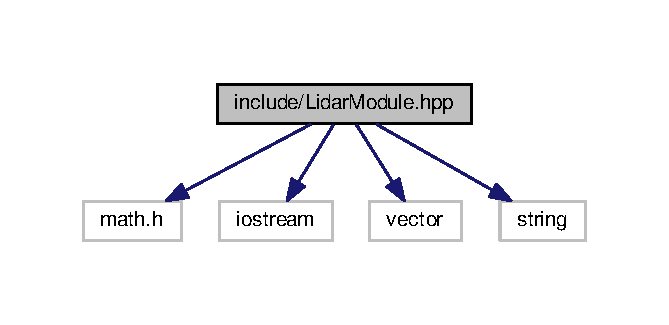
\includegraphics[width=321pt]{_lidar_module_8hpp__incl}
\end{center}
\end{figure}
This graph shows which files directly or indirectly include this file\+:
\nopagebreak
\begin{figure}[H]
\begin{center}
\leavevmode
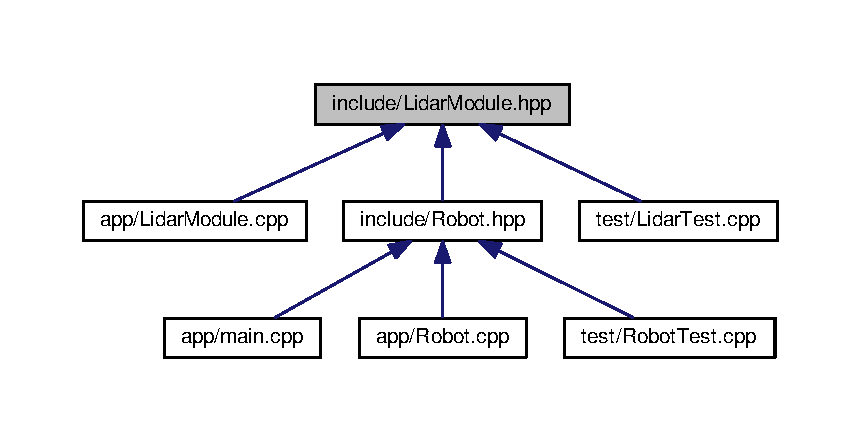
\includegraphics[width=350pt]{_lidar_module_8hpp__dep__incl}
\end{center}
\end{figure}
\subsection*{Classes}
\begin{DoxyCompactItemize}
\item 
class \hyperlink{class_lidar_module}{Lidar\+Module}
\begin{DoxyCompactList}\small\item\em Class for lidar module. \end{DoxyCompactList}\end{DoxyCompactItemize}


\subsection{Detailed Description}
E\+N\+P\+M808X, Midsemester project. 

\begin{DoxyAuthor}{Author}
Karan Vivek Bhargava 
\end{DoxyAuthor}
\begin{DoxyCopyright}{Copyright}
M\+IT License
\end{DoxyCopyright}
\hypertarget{_robot_test_8cpp_DESCRIPTION}{}\subsection{D\+E\+S\+C\+R\+I\+P\+T\+I\+ON}\label{_robot_test_8cpp_DESCRIPTION}
This program is controlling a robot\textquotesingle{}s heading direction using sensor fusion. 
\hypertarget{_path_planning_module_8hpp}{}\section{include/\+Path\+Planning\+Module.hpp File Reference}
\label{_path_planning_module_8hpp}\index{include/\+Path\+Planning\+Module.\+hpp@{include/\+Path\+Planning\+Module.\+hpp}}


E\+N\+P\+M808X, Midsemester project.  


{\ttfamily \#include $<$iostream$>$}\\*
{\ttfamily \#include $<$vector$>$}\\*
{\ttfamily \#include $<$algorithm$>$}\\*
Include dependency graph for Path\+Planning\+Module.\+hpp\+:
\nopagebreak
\begin{figure}[H]
\begin{center}
\leavevmode
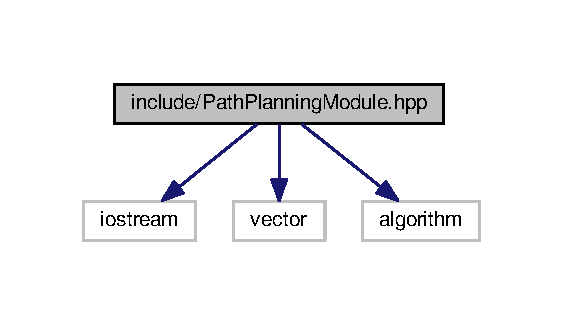
\includegraphics[width=270pt]{_path_planning_module_8hpp__incl}
\end{center}
\end{figure}
This graph shows which files directly or indirectly include this file\+:
\nopagebreak
\begin{figure}[H]
\begin{center}
\leavevmode
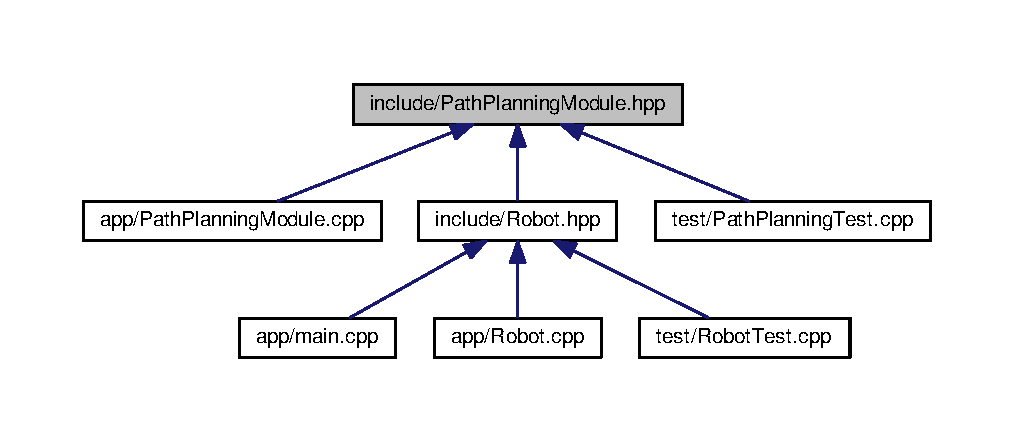
\includegraphics[width=350pt]{_path_planning_module_8hpp__dep__incl}
\end{center}
\end{figure}
\subsection*{Classes}
\begin{DoxyCompactItemize}
\item 
class \hyperlink{class_path_planning_module}{Path\+Planning\+Module}
\begin{DoxyCompactList}\small\item\em Class for path planning module. \end{DoxyCompactList}\end{DoxyCompactItemize}


\subsection{Detailed Description}
E\+N\+P\+M808X, Midsemester project. 

\begin{DoxyAuthor}{Author}
Karan Vivek Bhargava 
\end{DoxyAuthor}
\begin{DoxyCopyright}{Copyright}
M\+IT License
\end{DoxyCopyright}
\hypertarget{_path_planning_test_8cpp_DESCRIPTION}{}\subsection{D\+E\+S\+C\+R\+I\+P\+T\+I\+ON}\label{_path_planning_test_8cpp_DESCRIPTION}
This program is controlling a robot\textquotesingle{}s heading direction using sensor fusion. 
\hypertarget{_robot_8hpp}{}\section{include/\+Robot.hpp File Reference}
\label{_robot_8hpp}\index{include/\+Robot.\+hpp@{include/\+Robot.\+hpp}}


E\+N\+P\+M808X, Midsemester project.  


{\ttfamily \#include $<$iostream$>$}\\*
{\ttfamily \#include $<$vector$>$}\\*
{\ttfamily \#include $<$string$>$}\\*
{\ttfamily \#include \char`\"{}Camera\+Module.\+hpp\char`\"{}}\\*
{\ttfamily \#include \char`\"{}Path\+Planning\+Module.\+hpp\char`\"{}}\\*
{\ttfamily \#include \char`\"{}Lidar\+Module.\+hpp\char`\"{}}\\*
{\ttfamily \#include \char`\"{}Sensor\+Fusion\+Module.\+hpp\char`\"{}}\\*
Include dependency graph for Robot.\+hpp\+:
\nopagebreak
\begin{figure}[H]
\begin{center}
\leavevmode
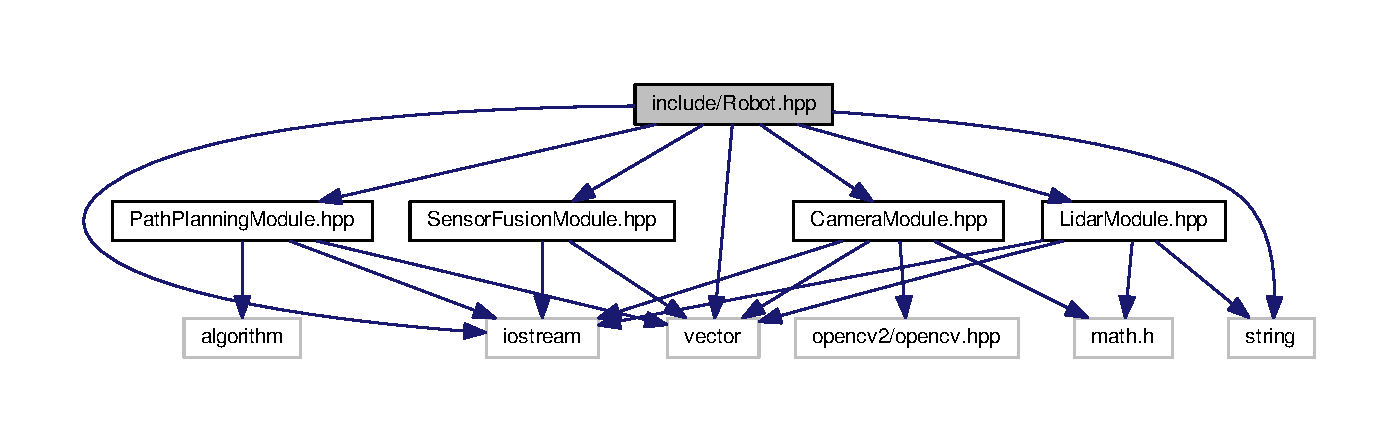
\includegraphics[width=350pt]{_robot_8hpp__incl}
\end{center}
\end{figure}
This graph shows which files directly or indirectly include this file\+:
\nopagebreak
\begin{figure}[H]
\begin{center}
\leavevmode
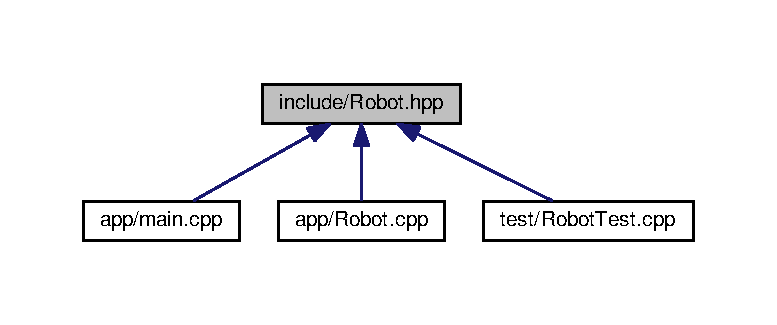
\includegraphics[width=350pt]{_robot_8hpp__dep__incl}
\end{center}
\end{figure}
\subsection*{Classes}
\begin{DoxyCompactItemize}
\item 
class \hyperlink{class_robot}{Robot}
\begin{DoxyCompactList}\small\item\em Class for robot. \end{DoxyCompactList}\end{DoxyCompactItemize}


\subsection{Detailed Description}
E\+N\+P\+M808X, Midsemester project. 

\begin{DoxyAuthor}{Author}
Karan Vivek Bhargava 
\end{DoxyAuthor}
\begin{DoxyCopyright}{Copyright}
M\+IT License
\end{DoxyCopyright}
\hypertarget{_robot_test_8cpp_DESCRIPTION}{}\subsection{D\+E\+S\+C\+R\+I\+P\+T\+I\+ON}\label{_robot_test_8cpp_DESCRIPTION}
This program is controlling a robot\textquotesingle{}s heading direction using sensor fusion. 
\hypertarget{_sensor_fusion_module_8hpp}{}\section{include/\+Sensor\+Fusion\+Module.hpp File Reference}
\label{_sensor_fusion_module_8hpp}\index{include/\+Sensor\+Fusion\+Module.\+hpp@{include/\+Sensor\+Fusion\+Module.\+hpp}}


E\+N\+P\+M808X, Midsemester project.  


{\ttfamily \#include $<$iostream$>$}\\*
{\ttfamily \#include $<$vector$>$}\\*
Include dependency graph for Sensor\+Fusion\+Module.\+hpp\+:
\nopagebreak
\begin{figure}[H]
\begin{center}
\leavevmode
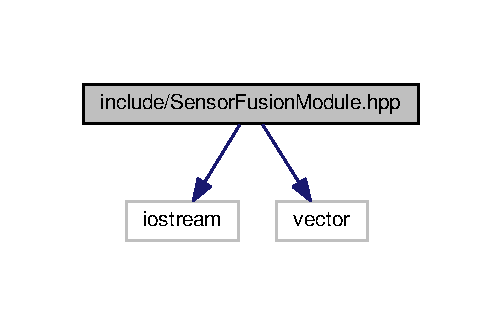
\includegraphics[width=241pt]{_sensor_fusion_module_8hpp__incl}
\end{center}
\end{figure}
This graph shows which files directly or indirectly include this file\+:
\nopagebreak
\begin{figure}[H]
\begin{center}
\leavevmode
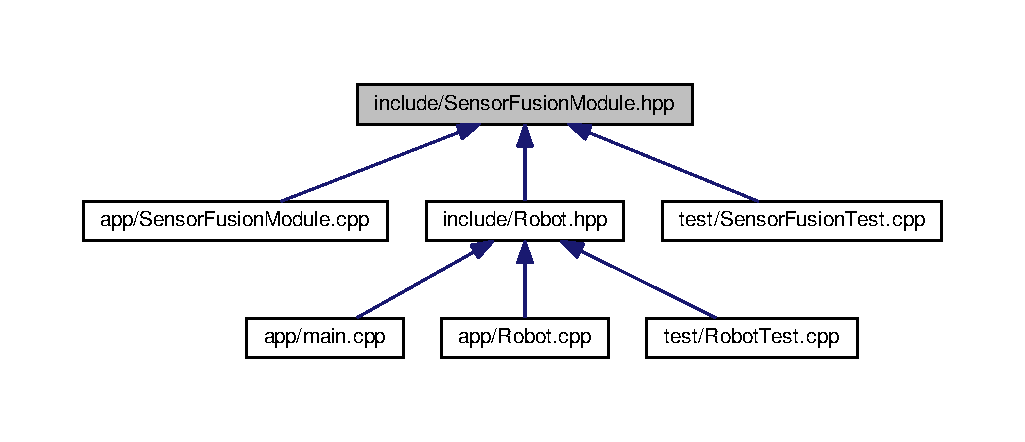
\includegraphics[width=350pt]{_sensor_fusion_module_8hpp__dep__incl}
\end{center}
\end{figure}
\subsection*{Classes}
\begin{DoxyCompactItemize}
\item 
class \hyperlink{class_sensor_fusion_module}{Sensor\+Fusion\+Module}
\begin{DoxyCompactList}\small\item\em Class for sensor fusion module. \end{DoxyCompactList}\end{DoxyCompactItemize}


\subsection{Detailed Description}
E\+N\+P\+M808X, Midsemester project. 

\begin{DoxyAuthor}{Author}
Karan Vivek Bhargava 
\end{DoxyAuthor}
\begin{DoxyCopyright}{Copyright}
M\+IT License
\end{DoxyCopyright}
\hypertarget{_path_planning_test_8cpp_DESCRIPTION}{}\subsection{D\+E\+S\+C\+R\+I\+P\+T\+I\+ON}\label{_path_planning_test_8cpp_DESCRIPTION}
This program is controlling a robot\textquotesingle{}s heading direction using sensor fusion. 
\hypertarget{readme_8md}{}\section{readme.\+md File Reference}
\label{readme_8md}\index{readme.\+md@{readme.\+md}}

\hypertarget{_camera_test_8cpp}{}\section{test/\+Camera\+Test.cpp File Reference}
\label{_camera_test_8cpp}\index{test/\+Camera\+Test.\+cpp@{test/\+Camera\+Test.\+cpp}}


E\+N\+P\+M808X, Midsemester project.  


{\ttfamily \#include $<$gtest/gtest.\+h$>$}\\*
{\ttfamily \#include $<$memory$>$}\\*
{\ttfamily \#include $<$vector$>$}\\*
{\ttfamily \#include \char`\"{}Camera\+Module.\+hpp\char`\"{}}\\*
Include dependency graph for Camera\+Test.\+cpp\+:
\nopagebreak
\begin{figure}[H]
\begin{center}
\leavevmode
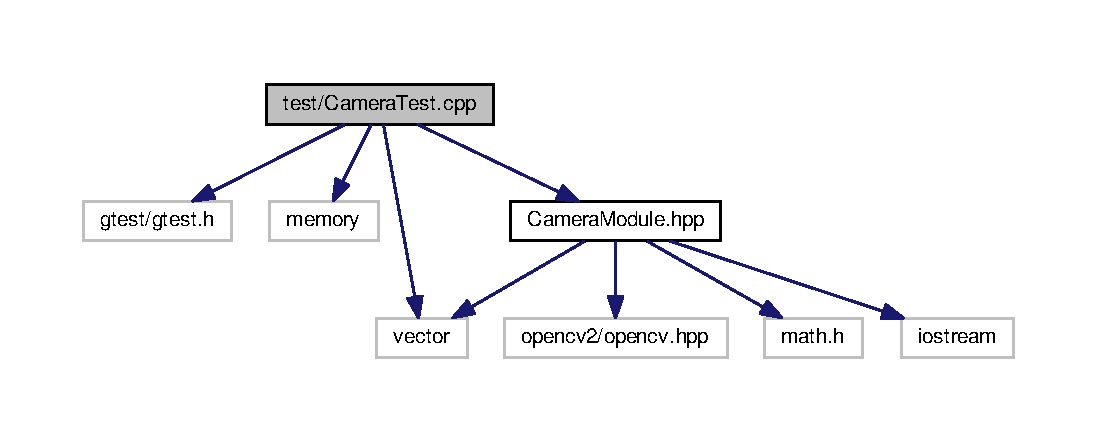
\includegraphics[width=350pt]{_camera_test_8cpp__incl}
\end{center}
\end{figure}
\subsection*{Classes}
\begin{DoxyCompactItemize}
\item 
class \hyperlink{class_camera_test}{Camera\+Test}
\begin{DoxyCompactList}\small\item\em Class for camera test. \end{DoxyCompactList}\end{DoxyCompactItemize}
\subsection*{Functions}
\begin{DoxyCompactItemize}
\item 
\hyperlink{_camera_test_8cpp_a688f0a01fbdc315f4e8f630e021e1926}{T\+E\+S\+T\+\_\+F} (\hyperlink{class_camera_test}{Camera\+Test}, Sanity\+Check)
\begin{DoxyCompactList}\small\item\em Test for Sanity, just checks whether everything is in order. \end{DoxyCompactList}\item 
\hyperlink{_camera_test_8cpp_a97f1bbd84e473ae9f230e21ea286a01b}{T\+E\+S\+T\+\_\+F} (\hyperlink{class_camera_test}{Camera\+Test}, Diagnostics\+Check)
\begin{DoxyCompactList}\small\item\em Run diagnostics test. \end{DoxyCompactList}\item 
\hyperlink{_camera_test_8cpp_a74c0f9c339aed622446321d1f2421900}{T\+E\+S\+T\+\_\+F} (\hyperlink{class_camera_test}{Camera\+Test}, Compute\+Probabilities\+Check)
\begin{DoxyCompactList}\small\item\em Run probability test. \end{DoxyCompactList}\end{DoxyCompactItemize}


\subsection{Detailed Description}
E\+N\+P\+M808X, Midsemester project. 

\begin{DoxyAuthor}{Author}
Karan Vivek Bhargava 
\end{DoxyAuthor}
\begin{DoxyCopyright}{Copyright}
M\+IT License
\end{DoxyCopyright}
\hypertarget{_robot_test_8cpp_DESCRIPTION}{}\subsection{D\+E\+S\+C\+R\+I\+P\+T\+I\+ON}\label{_robot_test_8cpp_DESCRIPTION}
This program is testing the camera module. 

\subsection{Function Documentation}
\index{Camera\+Test.\+cpp@{Camera\+Test.\+cpp}!T\+E\+S\+T\+\_\+F@{T\+E\+S\+T\+\_\+F}}
\index{T\+E\+S\+T\+\_\+F@{T\+E\+S\+T\+\_\+F}!Camera\+Test.\+cpp@{Camera\+Test.\+cpp}}
\subsubsection[{\texorpdfstring{T\+E\+S\+T\+\_\+\+F(\+Camera\+Test, Sanity\+Check)}{TEST_F(CameraTest, SanityCheck)}}]{\setlength{\rightskip}{0pt plus 5cm}T\+E\+S\+T\+\_\+F (
\begin{DoxyParamCaption}
\item[{{\bf Camera\+Test}}]{, }
\item[{Sanity\+Check}]{}
\end{DoxyParamCaption}
)}\hypertarget{_camera_test_8cpp_a688f0a01fbdc315f4e8f630e021e1926}{}\label{_camera_test_8cpp_a688f0a01fbdc315f4e8f630e021e1926}


Test for Sanity, just checks whether everything is in order. 

\index{Camera\+Test.\+cpp@{Camera\+Test.\+cpp}!T\+E\+S\+T\+\_\+F@{T\+E\+S\+T\+\_\+F}}
\index{T\+E\+S\+T\+\_\+F@{T\+E\+S\+T\+\_\+F}!Camera\+Test.\+cpp@{Camera\+Test.\+cpp}}
\subsubsection[{\texorpdfstring{T\+E\+S\+T\+\_\+\+F(\+Camera\+Test, Diagnostics\+Check)}{TEST_F(CameraTest, DiagnosticsCheck)}}]{\setlength{\rightskip}{0pt plus 5cm}T\+E\+S\+T\+\_\+F (
\begin{DoxyParamCaption}
\item[{{\bf Camera\+Test}}]{, }
\item[{Diagnostics\+Check}]{}
\end{DoxyParamCaption}
)}\hypertarget{_camera_test_8cpp_a97f1bbd84e473ae9f230e21ea286a01b}{}\label{_camera_test_8cpp_a97f1bbd84e473ae9f230e21ea286a01b}


Run diagnostics test. 


\begin{DoxyParams}[1]{Parameters}
\mbox{\tt in}  & {\em \hyperlink{class_camera_test}{Camera\+Test}} & cam object \\
\hline
\mbox{\tt in}  & {\em Diagnostics\+Check} & Name of the test \\
\hline
\end{DoxyParams}
\index{Camera\+Test.\+cpp@{Camera\+Test.\+cpp}!T\+E\+S\+T\+\_\+F@{T\+E\+S\+T\+\_\+F}}
\index{T\+E\+S\+T\+\_\+F@{T\+E\+S\+T\+\_\+F}!Camera\+Test.\+cpp@{Camera\+Test.\+cpp}}
\subsubsection[{\texorpdfstring{T\+E\+S\+T\+\_\+\+F(\+Camera\+Test, Compute\+Probabilities\+Check)}{TEST_F(CameraTest, ComputeProbabilitiesCheck)}}]{\setlength{\rightskip}{0pt plus 5cm}T\+E\+S\+T\+\_\+F (
\begin{DoxyParamCaption}
\item[{{\bf Camera\+Test}}]{, }
\item[{Compute\+Probabilities\+Check}]{}
\end{DoxyParamCaption}
)}\hypertarget{_camera_test_8cpp_a74c0f9c339aed622446321d1f2421900}{}\label{_camera_test_8cpp_a74c0f9c339aed622446321d1f2421900}


Run probability test. 


\begin{DoxyParams}[1]{Parameters}
\mbox{\tt in}  & {\em \hyperlink{class_camera_test}{Camera\+Test}} & cam object \\
\hline
\mbox{\tt in}  & {\em Compute\+Probabilities\+Check} & Name of the test \\
\hline
\end{DoxyParams}

\hypertarget{_lidar_test_8cpp}{}\section{test/\+Lidar\+Test.cpp File Reference}
\label{_lidar_test_8cpp}\index{test/\+Lidar\+Test.\+cpp@{test/\+Lidar\+Test.\+cpp}}


E\+N\+P\+M808X, Midsemester project.  


{\ttfamily \#include $<$gtest/gtest.\+h$>$}\\*
{\ttfamily \#include $<$memory$>$}\\*
{\ttfamily \#include $<$vector$>$}\\*
{\ttfamily \#include \char`\"{}Lidar\+Module.\+hpp\char`\"{}}\\*
Include dependency graph for Lidar\+Test.\+cpp\+:
\nopagebreak
\begin{figure}[H]
\begin{center}
\leavevmode
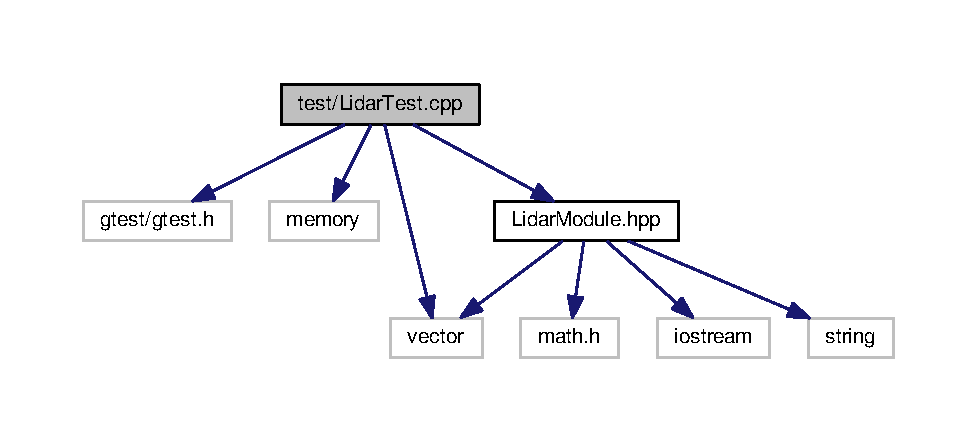
\includegraphics[width=350pt]{_lidar_test_8cpp__incl}
\end{center}
\end{figure}
\subsection*{Classes}
\begin{DoxyCompactItemize}
\item 
class \hyperlink{class_lidar_test}{Lidar\+Test}
\begin{DoxyCompactList}\small\item\em Class for lidar test. \end{DoxyCompactList}\end{DoxyCompactItemize}
\subsection*{Functions}
\begin{DoxyCompactItemize}
\item 
\hyperlink{_lidar_test_8cpp_a0b4ba51165fbdd18f256988ca2315c13}{T\+E\+S\+T\+\_\+F} (\hyperlink{class_lidar_test}{Lidar\+Test}, Sanity\+Check)\hypertarget{_lidar_test_8cpp_a0b4ba51165fbdd18f256988ca2315c13}{}\label{_lidar_test_8cpp_a0b4ba51165fbdd18f256988ca2315c13}

\begin{DoxyCompactList}\small\item\em Test for Sanity, just checks whether everything is in order. \end{DoxyCompactList}\item 
\hyperlink{_lidar_test_8cpp_a6d07bbf2e3557456fb7c9f0f81f72658}{T\+E\+S\+T\+\_\+F} (\hyperlink{class_lidar_test}{Lidar\+Test}, Diagnostics\+Check)
\begin{DoxyCompactList}\small\item\em Run diagnostics test. \end{DoxyCompactList}\item 
\hyperlink{_lidar_test_8cpp_aadfb007adeb5cee56d3df08a92075a5a}{T\+E\+S\+T\+\_\+F} (\hyperlink{class_lidar_test}{Lidar\+Test}, Compute\+Probabilities\+Check)
\begin{DoxyCompactList}\small\item\em Run probability test. \end{DoxyCompactList}\end{DoxyCompactItemize}


\subsection{Detailed Description}
E\+N\+P\+M808X, Midsemester project. 

\begin{DoxyAuthor}{Author}
Karan Vivek Bhargava 
\end{DoxyAuthor}
\begin{DoxyCopyright}{Copyright}
M\+IT License
\end{DoxyCopyright}
\hypertarget{_path_planning_test_8cpp_DESCRIPTION}{}\subsection{D\+E\+S\+C\+R\+I\+P\+T\+I\+ON}\label{_path_planning_test_8cpp_DESCRIPTION}
This program is testing the lidar module. 

\subsection{Function Documentation}
\index{Lidar\+Test.\+cpp@{Lidar\+Test.\+cpp}!T\+E\+S\+T\+\_\+F@{T\+E\+S\+T\+\_\+F}}
\index{T\+E\+S\+T\+\_\+F@{T\+E\+S\+T\+\_\+F}!Lidar\+Test.\+cpp@{Lidar\+Test.\+cpp}}
\subsubsection[{\texorpdfstring{T\+E\+S\+T\+\_\+\+F(\+Lidar\+Test, Diagnostics\+Check)}{TEST_F(LidarTest, DiagnosticsCheck)}}]{\setlength{\rightskip}{0pt plus 5cm}T\+E\+S\+T\+\_\+F (
\begin{DoxyParamCaption}
\item[{{\bf Lidar\+Test}}]{, }
\item[{Diagnostics\+Check}]{}
\end{DoxyParamCaption}
)}\hypertarget{_lidar_test_8cpp_a6d07bbf2e3557456fb7c9f0f81f72658}{}\label{_lidar_test_8cpp_a6d07bbf2e3557456fb7c9f0f81f72658}


Run diagnostics test. 


\begin{DoxyParams}[1]{Parameters}
\mbox{\tt in}  & {\em \hyperlink{class_lidar_test}{Lidar\+Test}} & lidar object \\
\hline
\mbox{\tt in}  & {\em Diagnostics\+Check} & Name of the test \\
\hline
\end{DoxyParams}


Definition at line 41 of file Lidar\+Test.\+cpp.

\index{Lidar\+Test.\+cpp@{Lidar\+Test.\+cpp}!T\+E\+S\+T\+\_\+F@{T\+E\+S\+T\+\_\+F}}
\index{T\+E\+S\+T\+\_\+F@{T\+E\+S\+T\+\_\+F}!Lidar\+Test.\+cpp@{Lidar\+Test.\+cpp}}
\subsubsection[{\texorpdfstring{T\+E\+S\+T\+\_\+\+F(\+Lidar\+Test, Compute\+Probabilities\+Check)}{TEST_F(LidarTest, ComputeProbabilitiesCheck)}}]{\setlength{\rightskip}{0pt plus 5cm}T\+E\+S\+T\+\_\+F (
\begin{DoxyParamCaption}
\item[{{\bf Lidar\+Test}}]{, }
\item[{Compute\+Probabilities\+Check}]{}
\end{DoxyParamCaption}
)}\hypertarget{_lidar_test_8cpp_aadfb007adeb5cee56d3df08a92075a5a}{}\label{_lidar_test_8cpp_aadfb007adeb5cee56d3df08a92075a5a}


Run probability test. 


\begin{DoxyParams}[1]{Parameters}
\mbox{\tt in}  & {\em \hyperlink{class_lidar_test}{Lidar\+Test}} & lidar object \\
\hline
\mbox{\tt in}  & {\em Compute\+Probabilities\+Check} & Name of the test \\
\hline
\end{DoxyParams}


Definition at line 52 of file Lidar\+Test.\+cpp.


\hypertarget{_path_planning_test_8cpp}{}\section{test/\+Path\+Planning\+Test.cpp File Reference}
\label{_path_planning_test_8cpp}\index{test/\+Path\+Planning\+Test.\+cpp@{test/\+Path\+Planning\+Test.\+cpp}}


E\+N\+P\+M808X, Midsemester project.  


{\ttfamily \#include $<$gtest/gtest.\+h$>$}\\*
{\ttfamily \#include $<$memory$>$}\\*
{\ttfamily \#include $<$vector$>$}\\*
{\ttfamily \#include \char`\"{}Path\+Planning\+Module.\+hpp\char`\"{}}\\*
Include dependency graph for Path\+Planning\+Test.\+cpp\+:
\nopagebreak
\begin{figure}[H]
\begin{center}
\leavevmode
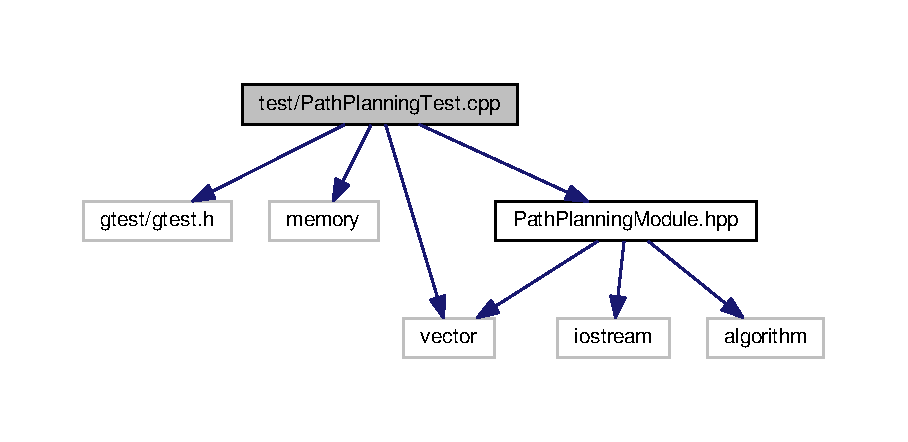
\includegraphics[width=350pt]{_path_planning_test_8cpp__incl}
\end{center}
\end{figure}
\subsection*{Classes}
\begin{DoxyCompactItemize}
\item 
class \hyperlink{class_path_planning_test}{Path\+Planning\+Test}
\begin{DoxyCompactList}\small\item\em Class for path planning test. \end{DoxyCompactList}\end{DoxyCompactItemize}
\subsection*{Functions}
\begin{DoxyCompactItemize}
\item 
\hyperlink{_path_planning_test_8cpp_a8a452f61ca0efedbc8b5ef1bb02c24c5}{T\+E\+S\+T\+\_\+F} (\hyperlink{class_path_planning_test}{Path\+Planning\+Test}, Sanity\+Check)\hypertarget{_path_planning_test_8cpp_a8a452f61ca0efedbc8b5ef1bb02c24c5}{}\label{_path_planning_test_8cpp_a8a452f61ca0efedbc8b5ef1bb02c24c5}

\begin{DoxyCompactList}\small\item\em Test for Sanity, just checks whether everything is in order. \end{DoxyCompactList}\item 
\hyperlink{_path_planning_test_8cpp_a14ec3b31967e7f539dbf9dd67747754c}{T\+E\+S\+T\+\_\+F} (\hyperlink{class_path_planning_test}{Path\+Planning\+Test}, Diagnostics\+Check)
\begin{DoxyCompactList}\small\item\em Run diagnostics test. \end{DoxyCompactList}\item 
\hyperlink{_path_planning_test_8cpp_a1c773393dcf781b7cac2a7b57ab37bbb}{T\+E\+S\+T\+\_\+F} (\hyperlink{class_path_planning_test}{Path\+Planning\+Test}, Set\+Direction\+Check)
\begin{DoxyCompactList}\small\item\em Test for whether the direction is set or not. \end{DoxyCompactList}\item 
\hyperlink{_path_planning_test_8cpp_ae2eb0a8f62e308fb067d14f55af996ef}{T\+E\+S\+T\+\_\+F} (\hyperlink{class_path_planning_test}{Path\+Planning\+Test}, Modification\+Check)
\begin{DoxyCompactList}\small\item\em Test for whether the direction is modified. \end{DoxyCompactList}\end{DoxyCompactItemize}


\subsection{Detailed Description}
E\+N\+P\+M808X, Midsemester project. 

\begin{DoxyAuthor}{Author}
Karan Vivek Bhargava 
\end{DoxyAuthor}
\begin{DoxyCopyright}{Copyright}
M\+IT License
\end{DoxyCopyright}
\hypertarget{_path_planning_test_8cpp_DESCRIPTION}{}\subsection{D\+E\+S\+C\+R\+I\+P\+T\+I\+ON}\label{_path_planning_test_8cpp_DESCRIPTION}
This program is testing the path planning module. 

\subsection{Function Documentation}
\index{Path\+Planning\+Test.\+cpp@{Path\+Planning\+Test.\+cpp}!T\+E\+S\+T\+\_\+F@{T\+E\+S\+T\+\_\+F}}
\index{T\+E\+S\+T\+\_\+F@{T\+E\+S\+T\+\_\+F}!Path\+Planning\+Test.\+cpp@{Path\+Planning\+Test.\+cpp}}
\subsubsection[{\texorpdfstring{T\+E\+S\+T\+\_\+\+F(\+Path\+Planning\+Test, Diagnostics\+Check)}{TEST_F(PathPlanningTest, DiagnosticsCheck)}}]{\setlength{\rightskip}{0pt plus 5cm}T\+E\+S\+T\+\_\+F (
\begin{DoxyParamCaption}
\item[{{\bf Path\+Planning\+Test}}]{, }
\item[{Diagnostics\+Check}]{}
\end{DoxyParamCaption}
)}\hypertarget{_path_planning_test_8cpp_a14ec3b31967e7f539dbf9dd67747754c}{}\label{_path_planning_test_8cpp_a14ec3b31967e7f539dbf9dd67747754c}


Run diagnostics test. 


\begin{DoxyParams}[1]{Parameters}
\mbox{\tt in}  & {\em \hyperlink{class_path_planning_test}{Path\+Planning\+Test}} & path planning object \\
\hline
\mbox{\tt in}  & {\em Diagnostics\+Check} & Name of the test \\
\hline
\end{DoxyParams}


Definition at line 41 of file Path\+Planning\+Test.\+cpp.

\index{Path\+Planning\+Test.\+cpp@{Path\+Planning\+Test.\+cpp}!T\+E\+S\+T\+\_\+F@{T\+E\+S\+T\+\_\+F}}
\index{T\+E\+S\+T\+\_\+F@{T\+E\+S\+T\+\_\+F}!Path\+Planning\+Test.\+cpp@{Path\+Planning\+Test.\+cpp}}
\subsubsection[{\texorpdfstring{T\+E\+S\+T\+\_\+\+F(\+Path\+Planning\+Test, Set\+Direction\+Check)}{TEST_F(PathPlanningTest, SetDirectionCheck)}}]{\setlength{\rightskip}{0pt plus 5cm}T\+E\+S\+T\+\_\+F (
\begin{DoxyParamCaption}
\item[{{\bf Path\+Planning\+Test}}]{, }
\item[{Set\+Direction\+Check}]{}
\end{DoxyParamCaption}
)}\hypertarget{_path_planning_test_8cpp_a1c773393dcf781b7cac2a7b57ab37bbb}{}\label{_path_planning_test_8cpp_a1c773393dcf781b7cac2a7b57ab37bbb}


Test for whether the direction is set or not. 


\begin{DoxyParams}[1]{Parameters}
\mbox{\tt in}  & {\em \hyperlink{class_path_planning_test}{Path\+Planning\+Test}} & path planning object \\
\hline
\mbox{\tt in}  & {\em Set\+Direction\+Check} & Name of the test \\
\hline
\end{DoxyParams}


Definition at line 51 of file Path\+Planning\+Test.\+cpp.

\index{Path\+Planning\+Test.\+cpp@{Path\+Planning\+Test.\+cpp}!T\+E\+S\+T\+\_\+F@{T\+E\+S\+T\+\_\+F}}
\index{T\+E\+S\+T\+\_\+F@{T\+E\+S\+T\+\_\+F}!Path\+Planning\+Test.\+cpp@{Path\+Planning\+Test.\+cpp}}
\subsubsection[{\texorpdfstring{T\+E\+S\+T\+\_\+\+F(\+Path\+Planning\+Test, Modification\+Check)}{TEST_F(PathPlanningTest, ModificationCheck)}}]{\setlength{\rightskip}{0pt plus 5cm}T\+E\+S\+T\+\_\+F (
\begin{DoxyParamCaption}
\item[{{\bf Path\+Planning\+Test}}]{, }
\item[{Modification\+Check}]{}
\end{DoxyParamCaption}
)}\hypertarget{_path_planning_test_8cpp_ae2eb0a8f62e308fb067d14f55af996ef}{}\label{_path_planning_test_8cpp_ae2eb0a8f62e308fb067d14f55af996ef}


Test for whether the direction is modified. 


\begin{DoxyParams}[1]{Parameters}
\mbox{\tt in}  & {\em \hyperlink{class_path_planning_test}{Path\+Planning\+Test}} & path planning object \\
\hline
\mbox{\tt in}  & {\em Set\+Direction\+Check} & Name of the test \\
\hline
\end{DoxyParams}


Definition at line 62 of file Path\+Planning\+Test.\+cpp.


\hypertarget{_robot_test_8cpp}{}\section{test/\+Robot\+Test.cpp File Reference}
\label{_robot_test_8cpp}\index{test/\+Robot\+Test.\+cpp@{test/\+Robot\+Test.\+cpp}}


E\+N\+P\+M808X, Midsemester project.  


{\ttfamily \#include $<$gtest/gtest.\+h$>$}\\*
{\ttfamily \#include $<$memory$>$}\\*
{\ttfamily \#include $<$vector$>$}\\*
{\ttfamily \#include $<$string$>$}\\*
{\ttfamily \#include \char`\"{}Robot.\+hpp\char`\"{}}\\*
Include dependency graph for Robot\+Test.\+cpp\+:
\nopagebreak
\begin{figure}[H]
\begin{center}
\leavevmode
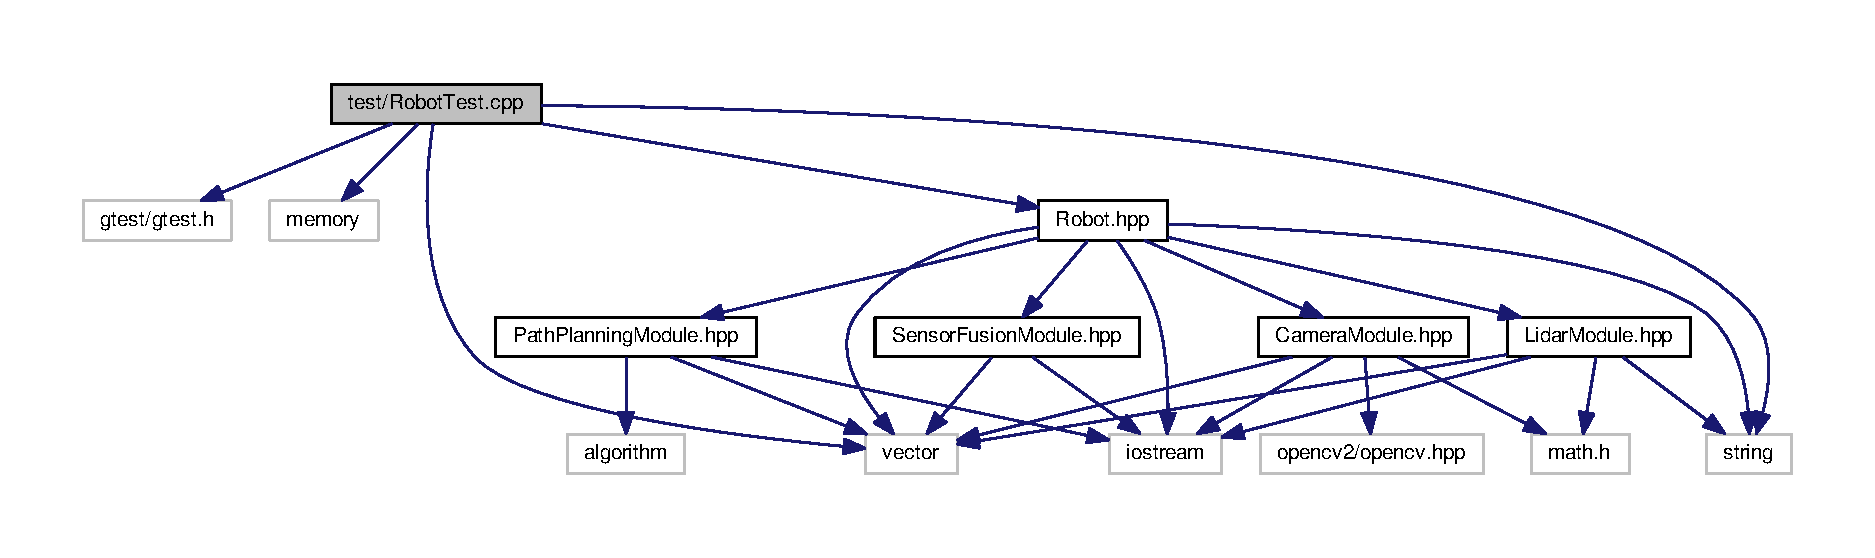
\includegraphics[width=350pt]{_robot_test_8cpp__incl}
\end{center}
\end{figure}
\subsection*{Classes}
\begin{DoxyCompactItemize}
\item 
class \hyperlink{class_robot_test}{Robot\+Test}
\begin{DoxyCompactList}\small\item\em Class for \hyperlink{class_robot}{Robot} test. \end{DoxyCompactList}\end{DoxyCompactItemize}
\subsection*{Functions}
\begin{DoxyCompactItemize}
\item 
\hyperlink{_robot_test_8cpp_a7b40cdf30b329ffe4da4e244f31a4b9f}{T\+E\+S\+T\+\_\+F} (\hyperlink{class_robot_test}{Robot\+Test}, Sanity\+Check)
\begin{DoxyCompactList}\small\item\em Test for Sanity, just checks whether everything is in order. \end{DoxyCompactList}\item 
\hyperlink{_robot_test_8cpp_a15d954307c6c224aadb68e501130ea2c}{T\+E\+S\+T\+\_\+F} (\hyperlink{class_robot_test}{Robot\+Test}, Diagnostics\+Check)
\begin{DoxyCompactList}\small\item\em Run diagnostics test. \end{DoxyCompactList}\item 
\hyperlink{_robot_test_8cpp_af26f65257a5839d805405daba1bc8e62}{T\+E\+S\+T\+\_\+F} (\hyperlink{class_robot_test}{Robot\+Test}, run\+Check)
\begin{DoxyCompactList}\small\item\em Test whether robot is running. \end{DoxyCompactList}\end{DoxyCompactItemize}


\subsection{Detailed Description}
E\+N\+P\+M808X, Midsemester project. 

\begin{DoxyAuthor}{Author}
Karan Vivek Bhargava 
\end{DoxyAuthor}
\begin{DoxyCopyright}{Copyright}
M\+IT License
\end{DoxyCopyright}
\hypertarget{_robot_test_8cpp_DESCRIPTION}{}\subsection{D\+E\+S\+C\+R\+I\+P\+T\+I\+ON}\label{_robot_test_8cpp_DESCRIPTION}
This program is testing the robot module. 

\subsection{Function Documentation}
\index{Robot\+Test.\+cpp@{Robot\+Test.\+cpp}!T\+E\+S\+T\+\_\+F@{T\+E\+S\+T\+\_\+F}}
\index{T\+E\+S\+T\+\_\+F@{T\+E\+S\+T\+\_\+F}!Robot\+Test.\+cpp@{Robot\+Test.\+cpp}}
\subsubsection[{\texorpdfstring{T\+E\+S\+T\+\_\+\+F(\+Robot\+Test, Sanity\+Check)}{TEST_F(RobotTest, SanityCheck)}}]{\setlength{\rightskip}{0pt plus 5cm}T\+E\+S\+T\+\_\+F (
\begin{DoxyParamCaption}
\item[{{\bf Robot\+Test}}]{, }
\item[{Sanity\+Check}]{}
\end{DoxyParamCaption}
)}\hypertarget{_robot_test_8cpp_a7b40cdf30b329ffe4da4e244f31a4b9f}{}\label{_robot_test_8cpp_a7b40cdf30b329ffe4da4e244f31a4b9f}


Test for Sanity, just checks whether everything is in order. 

\index{Robot\+Test.\+cpp@{Robot\+Test.\+cpp}!T\+E\+S\+T\+\_\+F@{T\+E\+S\+T\+\_\+F}}
\index{T\+E\+S\+T\+\_\+F@{T\+E\+S\+T\+\_\+F}!Robot\+Test.\+cpp@{Robot\+Test.\+cpp}}
\subsubsection[{\texorpdfstring{T\+E\+S\+T\+\_\+\+F(\+Robot\+Test, Diagnostics\+Check)}{TEST_F(RobotTest, DiagnosticsCheck)}}]{\setlength{\rightskip}{0pt plus 5cm}T\+E\+S\+T\+\_\+F (
\begin{DoxyParamCaption}
\item[{{\bf Robot\+Test}}]{, }
\item[{Diagnostics\+Check}]{}
\end{DoxyParamCaption}
)}\hypertarget{_robot_test_8cpp_a15d954307c6c224aadb68e501130ea2c}{}\label{_robot_test_8cpp_a15d954307c6c224aadb68e501130ea2c}


Run diagnostics test. 


\begin{DoxyParams}[1]{Parameters}
\mbox{\tt in}  & {\em \hyperlink{class_robot_test}{Robot\+Test}} & Contains all the objects \\
\hline
\mbox{\tt in}  & {\em Diagnostics\+Check} & Name of the test \\
\hline
\end{DoxyParams}
\index{Robot\+Test.\+cpp@{Robot\+Test.\+cpp}!T\+E\+S\+T\+\_\+F@{T\+E\+S\+T\+\_\+F}}
\index{T\+E\+S\+T\+\_\+F@{T\+E\+S\+T\+\_\+F}!Robot\+Test.\+cpp@{Robot\+Test.\+cpp}}
\subsubsection[{\texorpdfstring{T\+E\+S\+T\+\_\+\+F(\+Robot\+Test, run\+Check)}{TEST_F(RobotTest, runCheck)}}]{\setlength{\rightskip}{0pt plus 5cm}T\+E\+S\+T\+\_\+F (
\begin{DoxyParamCaption}
\item[{{\bf Robot\+Test}}]{, }
\item[{run\+Check}]{}
\end{DoxyParamCaption}
)}\hypertarget{_robot_test_8cpp_af26f65257a5839d805405daba1bc8e62}{}\label{_robot_test_8cpp_af26f65257a5839d805405daba1bc8e62}


Test whether robot is running. 


\begin{DoxyParams}[1]{Parameters}
\mbox{\tt in}  & {\em \hyperlink{class_robot_test}{Robot\+Test}} & Contains all the objects \\
\hline
\mbox{\tt in}  & {\em run\+Check} & Name of the test \\
\hline
\end{DoxyParams}

\hypertarget{_sensor_fusion_test_8cpp}{}\section{test/\+Sensor\+Fusion\+Test.cpp File Reference}
\label{_sensor_fusion_test_8cpp}\index{test/\+Sensor\+Fusion\+Test.\+cpp@{test/\+Sensor\+Fusion\+Test.\+cpp}}
{\ttfamily \#include $<$gtest/gtest.\+h$>$}\\*
{\ttfamily \#include $<$memory$>$}\\*
{\ttfamily \#include $<$vector$>$}\\*
{\ttfamily \#include \char`\"{}Sensor\+Fusion\+Module.\+hpp\char`\"{}}\\*
Include dependency graph for Sensor\+Fusion\+Test.\+cpp\+:
\nopagebreak
\begin{figure}[H]
\begin{center}
\leavevmode
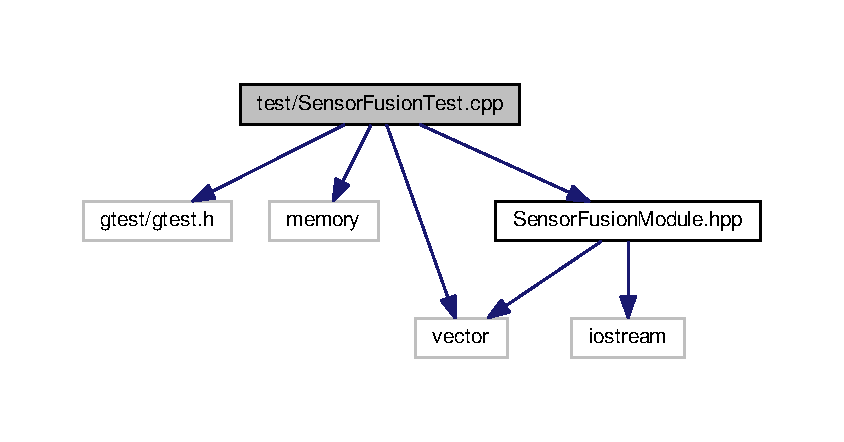
\includegraphics[width=350pt]{_sensor_fusion_test_8cpp__incl}
\end{center}
\end{figure}
\subsection*{Classes}
\begin{DoxyCompactItemize}
\item 
class \hyperlink{class_sensor_fusion_test}{Sensor\+Fusion\+Test}
\begin{DoxyCompactList}\small\item\em Class for sensor fusion test. \end{DoxyCompactList}\end{DoxyCompactItemize}
\subsection*{Functions}
\begin{DoxyCompactItemize}
\item 
\hyperlink{_sensor_fusion_test_8cpp_a39bffeecebf3cc056ec6476c2b28c6ec}{T\+E\+S\+T\+\_\+F} (\hyperlink{class_sensor_fusion_test}{Sensor\+Fusion\+Test}, Sanity\+Check)
\begin{DoxyCompactList}\small\item\em Test for Sanity, just checks whether everything is in order. \end{DoxyCompactList}\item 
\hyperlink{_sensor_fusion_test_8cpp_a1d85eb9167d4242ee94ff72ed37762fe}{T\+E\+S\+T\+\_\+F} (\hyperlink{class_sensor_fusion_test}{Sensor\+Fusion\+Test}, Diagnostics\+Check)
\begin{DoxyCompactList}\small\item\em Run diagnostics test. \end{DoxyCompactList}\item 
\hyperlink{_sensor_fusion_test_8cpp_a7baea4bfd6a786ee8ca00e7b77f5b6d5}{T\+E\+S\+T\+\_\+F} (\hyperlink{class_sensor_fusion_test}{Sensor\+Fusion\+Test}, Fusion\+Check)
\begin{DoxyCompactList}\small\item\em Run fusion test. \end{DoxyCompactList}\end{DoxyCompactItemize}


\subsection{Function Documentation}
\index{Sensor\+Fusion\+Test.\+cpp@{Sensor\+Fusion\+Test.\+cpp}!T\+E\+S\+T\+\_\+F@{T\+E\+S\+T\+\_\+F}}
\index{T\+E\+S\+T\+\_\+F@{T\+E\+S\+T\+\_\+F}!Sensor\+Fusion\+Test.\+cpp@{Sensor\+Fusion\+Test.\+cpp}}
\subsubsection[{\texorpdfstring{T\+E\+S\+T\+\_\+\+F(\+Sensor\+Fusion\+Test, Sanity\+Check)}{TEST_F(SensorFusionTest, SanityCheck)}}]{\setlength{\rightskip}{0pt plus 5cm}T\+E\+S\+T\+\_\+F (
\begin{DoxyParamCaption}
\item[{{\bf Sensor\+Fusion\+Test}}]{, }
\item[{Sanity\+Check}]{}
\end{DoxyParamCaption}
)}\hypertarget{_sensor_fusion_test_8cpp_a39bffeecebf3cc056ec6476c2b28c6ec}{}\label{_sensor_fusion_test_8cpp_a39bffeecebf3cc056ec6476c2b28c6ec}


Test for Sanity, just checks whether everything is in order. 

\index{Sensor\+Fusion\+Test.\+cpp@{Sensor\+Fusion\+Test.\+cpp}!T\+E\+S\+T\+\_\+F@{T\+E\+S\+T\+\_\+F}}
\index{T\+E\+S\+T\+\_\+F@{T\+E\+S\+T\+\_\+F}!Sensor\+Fusion\+Test.\+cpp@{Sensor\+Fusion\+Test.\+cpp}}
\subsubsection[{\texorpdfstring{T\+E\+S\+T\+\_\+\+F(\+Sensor\+Fusion\+Test, Diagnostics\+Check)}{TEST_F(SensorFusionTest, DiagnosticsCheck)}}]{\setlength{\rightskip}{0pt plus 5cm}T\+E\+S\+T\+\_\+F (
\begin{DoxyParamCaption}
\item[{{\bf Sensor\+Fusion\+Test}}]{, }
\item[{Diagnostics\+Check}]{}
\end{DoxyParamCaption}
)}\hypertarget{_sensor_fusion_test_8cpp_a1d85eb9167d4242ee94ff72ed37762fe}{}\label{_sensor_fusion_test_8cpp_a1d85eb9167d4242ee94ff72ed37762fe}


Run diagnostics test. 


\begin{DoxyParams}[1]{Parameters}
\mbox{\tt in}  & {\em \hyperlink{class_sensor_fusion_test}{Sensor\+Fusion\+Test}} & sensor fusion object \\
\hline
\mbox{\tt in}  & {\em Diagnostics\+Check} & Name of the test \\
\hline
\end{DoxyParams}
\index{Sensor\+Fusion\+Test.\+cpp@{Sensor\+Fusion\+Test.\+cpp}!T\+E\+S\+T\+\_\+F@{T\+E\+S\+T\+\_\+F}}
\index{T\+E\+S\+T\+\_\+F@{T\+E\+S\+T\+\_\+F}!Sensor\+Fusion\+Test.\+cpp@{Sensor\+Fusion\+Test.\+cpp}}
\subsubsection[{\texorpdfstring{T\+E\+S\+T\+\_\+\+F(\+Sensor\+Fusion\+Test, Fusion\+Check)}{TEST_F(SensorFusionTest, FusionCheck)}}]{\setlength{\rightskip}{0pt plus 5cm}T\+E\+S\+T\+\_\+F (
\begin{DoxyParamCaption}
\item[{{\bf Sensor\+Fusion\+Test}}]{, }
\item[{Fusion\+Check}]{}
\end{DoxyParamCaption}
)}\hypertarget{_sensor_fusion_test_8cpp_a7baea4bfd6a786ee8ca00e7b77f5b6d5}{}\label{_sensor_fusion_test_8cpp_a7baea4bfd6a786ee8ca00e7b77f5b6d5}


Run fusion test. 


\begin{DoxyParams}[1]{Parameters}
\mbox{\tt in}  & {\em \hyperlink{class_sensor_fusion_test}{Sensor\+Fusion\+Test}} & sensor fusion object \\
\hline
\mbox{\tt in}  & {\em Compute\+Probabilities\+Check} & Name of the test \\
\hline
\end{DoxyParams}

%--- End generated contents ---

% Index
\backmatter
\newpage
\phantomsection
\clearemptydoublepage
\addcontentsline{toc}{chapter}{Index}
\printindex

\end{document}
